%
% chapter.tex -- Kapitel über stetige Wavelet-Transformation
%
% (c) 2019 Prof Dr Andreas Müller, Hochschule Rapperswil
%
\chapter{Stetige Wavelet-Transformation
\label{chapter:cwt}}
Im Kapitel~\ref{chapter:haar-wavelet} wurde am Beispiel des Haar-Servlets
gezeigt, wie jede beliebige stetige Funktion als Linearkombination 
skalierten und verschobenen Versionen einer einzigen Ausgangsfunktion
$\psi(t)$ geschrieben werden kann.
Das Haar-Wavelet hat einen Ausweg aus der Schwierigkeit der
Fourier-Transformation gewiesen, Ereignisse sowohl auf der Zeitachse
wie auch bezüglich ihrer Frequenz zu lokalisieren.
Es bleibt aber eine Reihe von Schwierigkeiten, die vom Haar-Wavelet nicht
adressiert werden:
\begin{enumerate}
\item
Die Funktion $\psi$ ist nicht stetig, und alle daraus aufgebauten
Approximationsfunktionen sind nicht stetig
und erst recht nicht differenzierbar.
\item
Es werden nur Frequenzen verwendet, die $2^n$-fache einer Grundfrequenz
sind.
Die Analyse kann also nur Oktaven unterscheiden, während
Töne auf einer Tonleiter Frequenzverhältnisse von $\sqrt[12]{2}$ haben.
\end{enumerate}
Ziel dieses Kapitels ist, vernünftige Kriterien für Waveletfunktionen
$\psi(t)$ zu finden, so dass die Analyse und Synthese ähnlich einfach
wie für Haar-Wavelets möglich bleibt.
Ausserdem soll die stetige Wavelet-Transformation diskutiert werden,
welche das Problem der ``Zwischenfrequenzen'' löst.

% !TeX spellcheck = de_CH_frami

\section{Spectral Graph Wavelet Transformation\label{sec:sgwt:wavelets}}
\rhead{SGWT}

Hier wollen wir nun das Bisherige zur Spectral Graph Wavelet Transformation 
vereinen.

\subsection{Graph Fourier Transformation\label{subsec:sgwt:gft}}

Bevor wir uns auf die Graph Wavelets st\"urzen, wollen wir zuerst versuchen die 
Fourier Theorie auf Funktionen auf Graphen anzuwenden. Dazu nehmen wir das 
Beispiel eines Dirac-Stosses $\delta(x)$, siehe~\cref{fig:sgwt:gft:dirac}.
\begin{figure}
    \centering
    \begin{minipage}[b]{0.49\textwidth}
    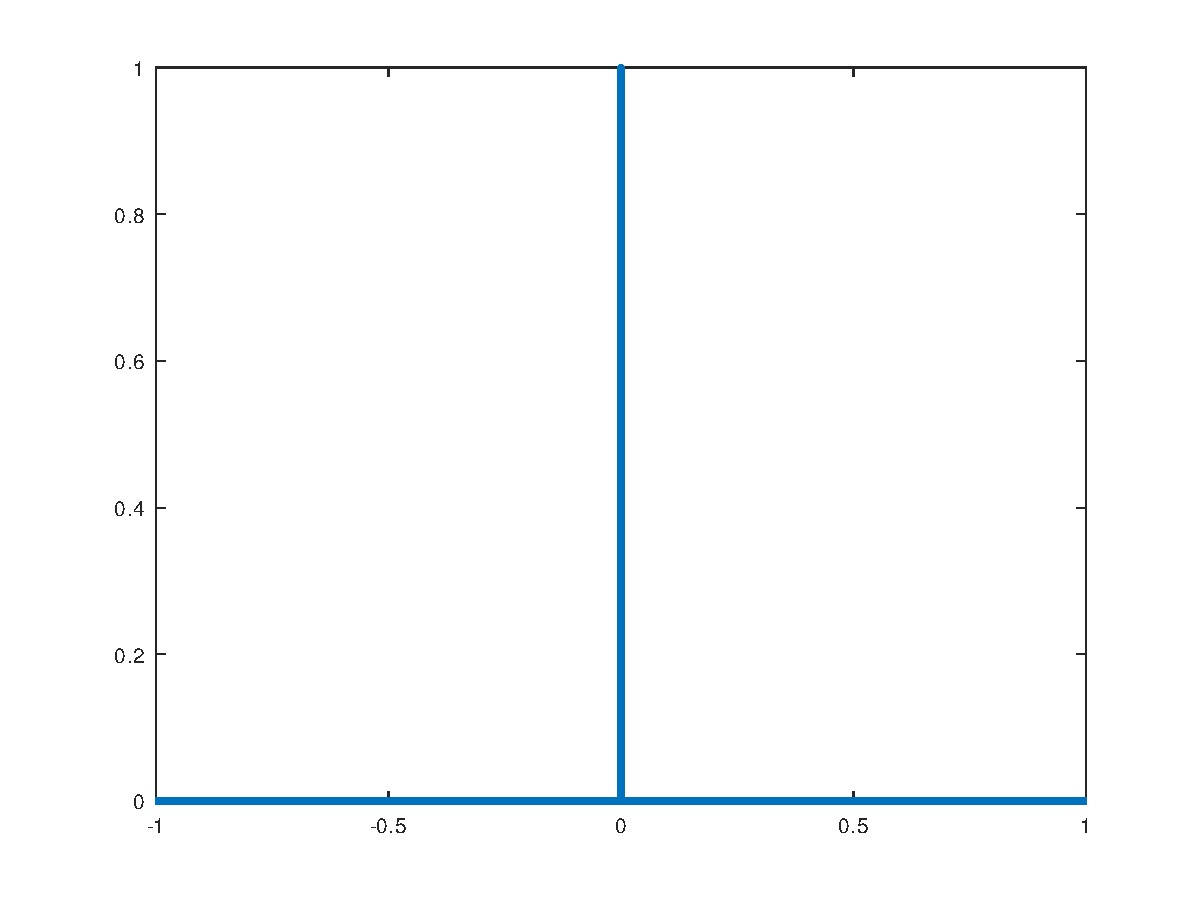
\includegraphics[
    width=\textwidth
    ]{papers/sgwt/images/dirac/dirac_delta.pdf}
    \vspace{-0pt}
    \caption{Darstellung eines Dirac-Stoss $\delta(x)$ mit maximal Wert $1$. 
        \label{fig:sgwt:gft:dirac}}
    \end{minipage}
    ~
    \begin{minipage}[b]{0.49\textwidth}
    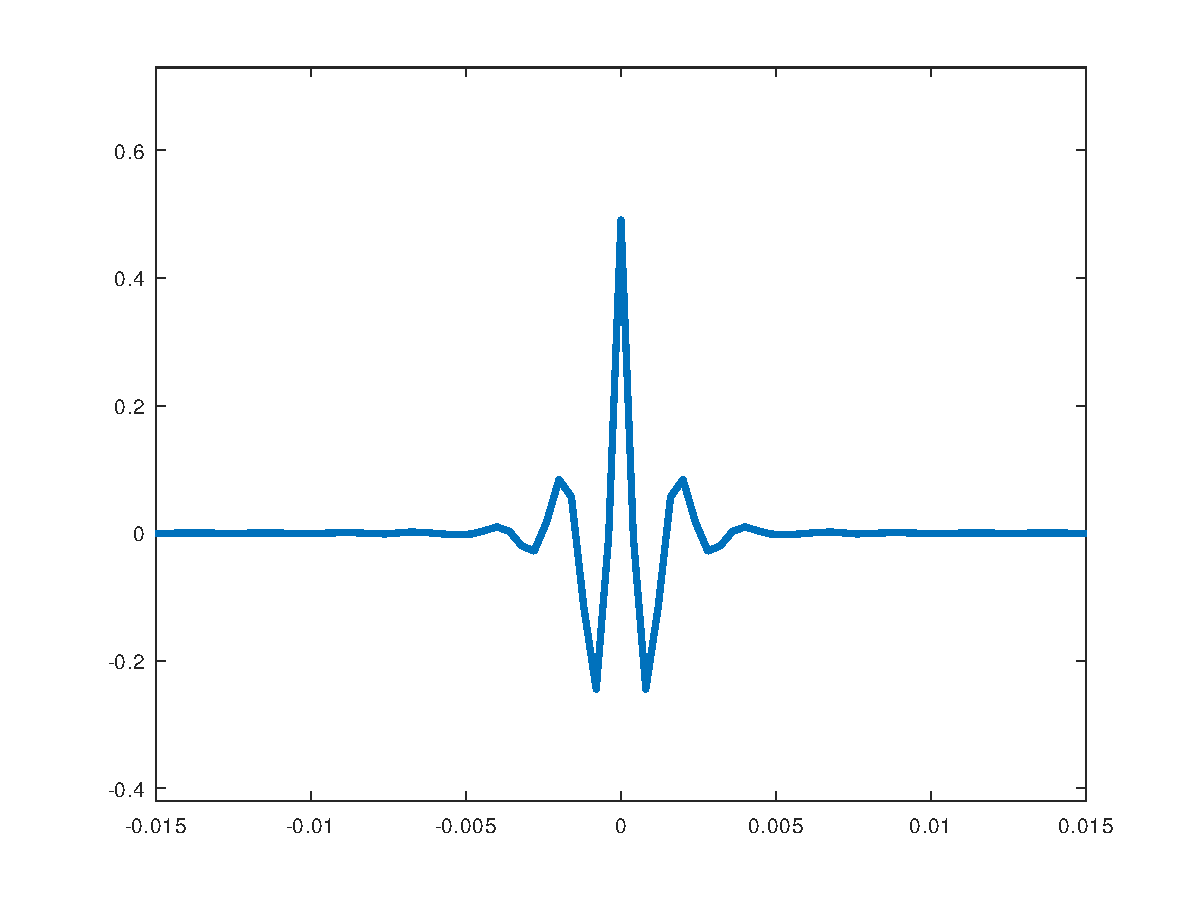
\includegraphics[
    width=\textwidth
    ]{papers/sgwt/images/dirac/dirac_g_igft.pdf}
    \vspace{-0pt}
    \caption{Fourier Transformation des Dirac-Stosses $\hat{\delta(x)}$ 
        aus~\cref{fig:sgwt:gft:dirac}.\label{fig:sgwt:gft:igft}}
    \end{minipage}
    ~
    \begin{minipage}[b]{0.49\textwidth}
    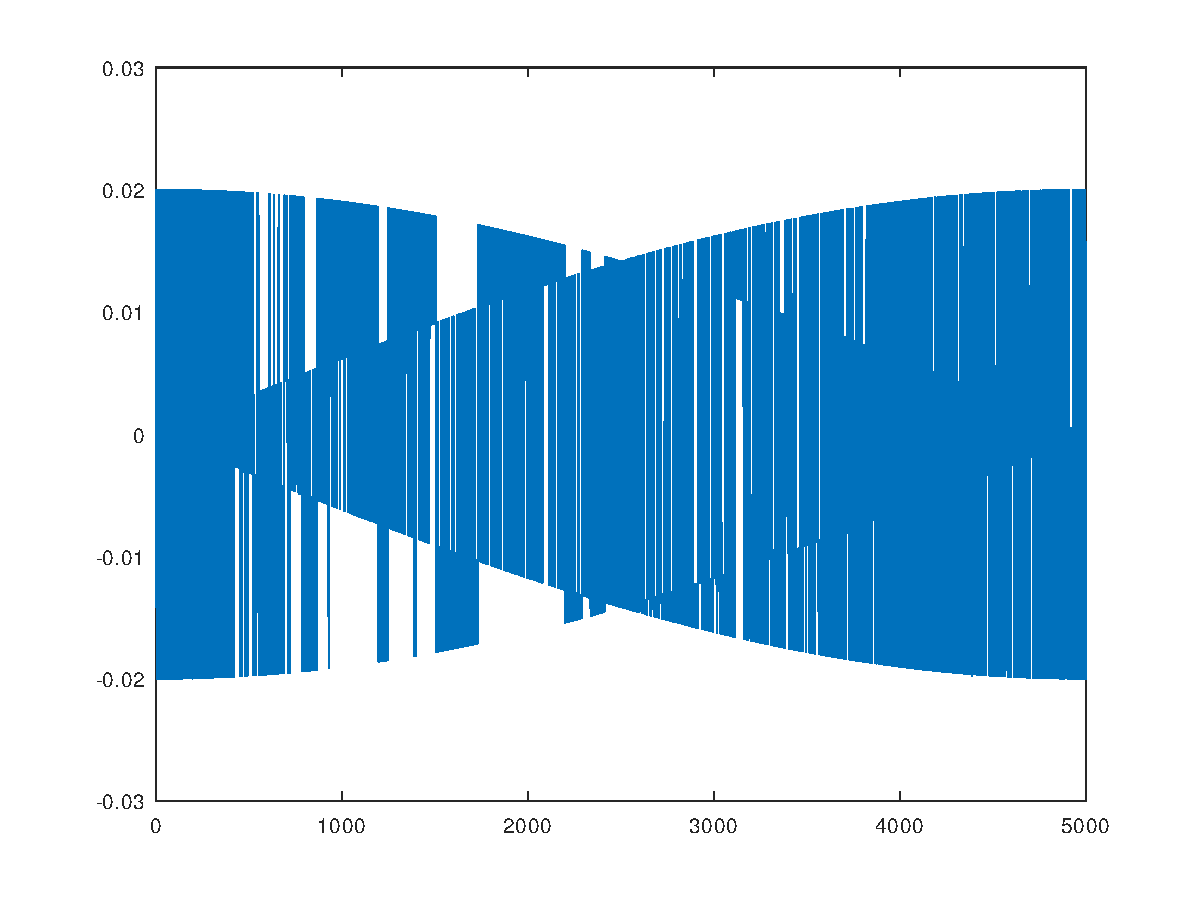
\includegraphics[
    width=\textwidth
    ]{papers/sgwt/images/dirac/dirac_gft.pdf}
    \vspace{-0pt}
    \caption{Fourier Transformation des Dirac-Stosses $\hat{\delta(x)}$ 
        aus~\cref{fig:sgwt:gft:dirac}.\label{fig:sgwt:gft:gft}}
    \end{minipage}
    ~
    \begin{minipage}[b]{0.49\textwidth}
    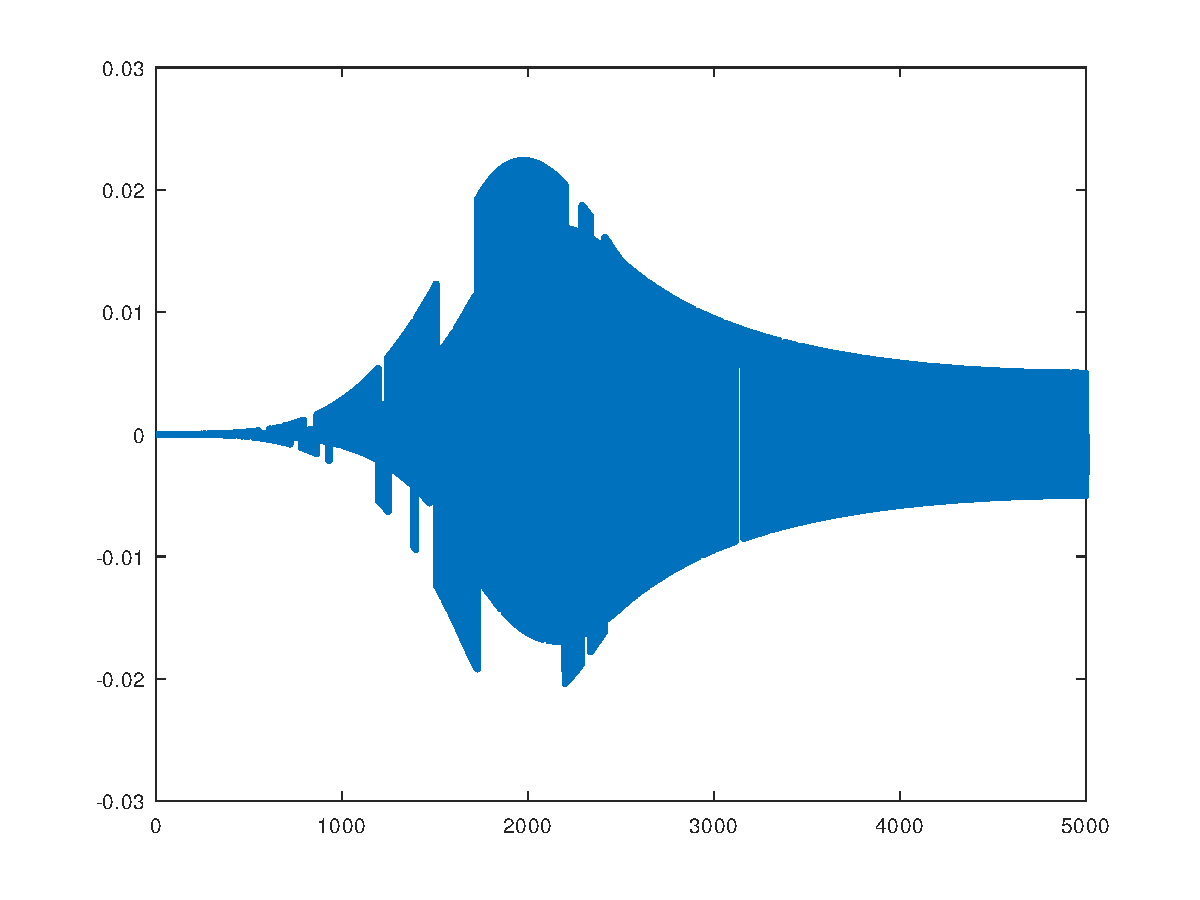
\includegraphics[
    width=\textwidth
    ]{papers/sgwt/images/dirac/dirac_g_gft.pdf}
    \vspace{-0pt}
    \caption{Fourier Transformation des Dirac-Stosses $\hat{\delta(x)}$ 
        aus~\cref{fig:sgwt:gft:dirac}.\label{fig:sgwt:gft:ggft}}
    \end{minipage}
\end{figure}
Wenn wir davon die Fourier Transformation berechnen, zu sehen 
in~\cref{fig:sgwt:gft:fftdirac}, stellen wir fest, das nicht nur alle 
Frequenzen vorhanden sondern auch alle gleich stark vorhanden sind. Die 
Fouriertransformierte $\hat{\delta}$ ist somit vollst\"andig delokalisiert.

$g(\lambda)\cdot\hat{\delta}(\lambda)$

\begin{figure}
    \centering
    \begin{minipage}[b]{0.49\textwidth}
    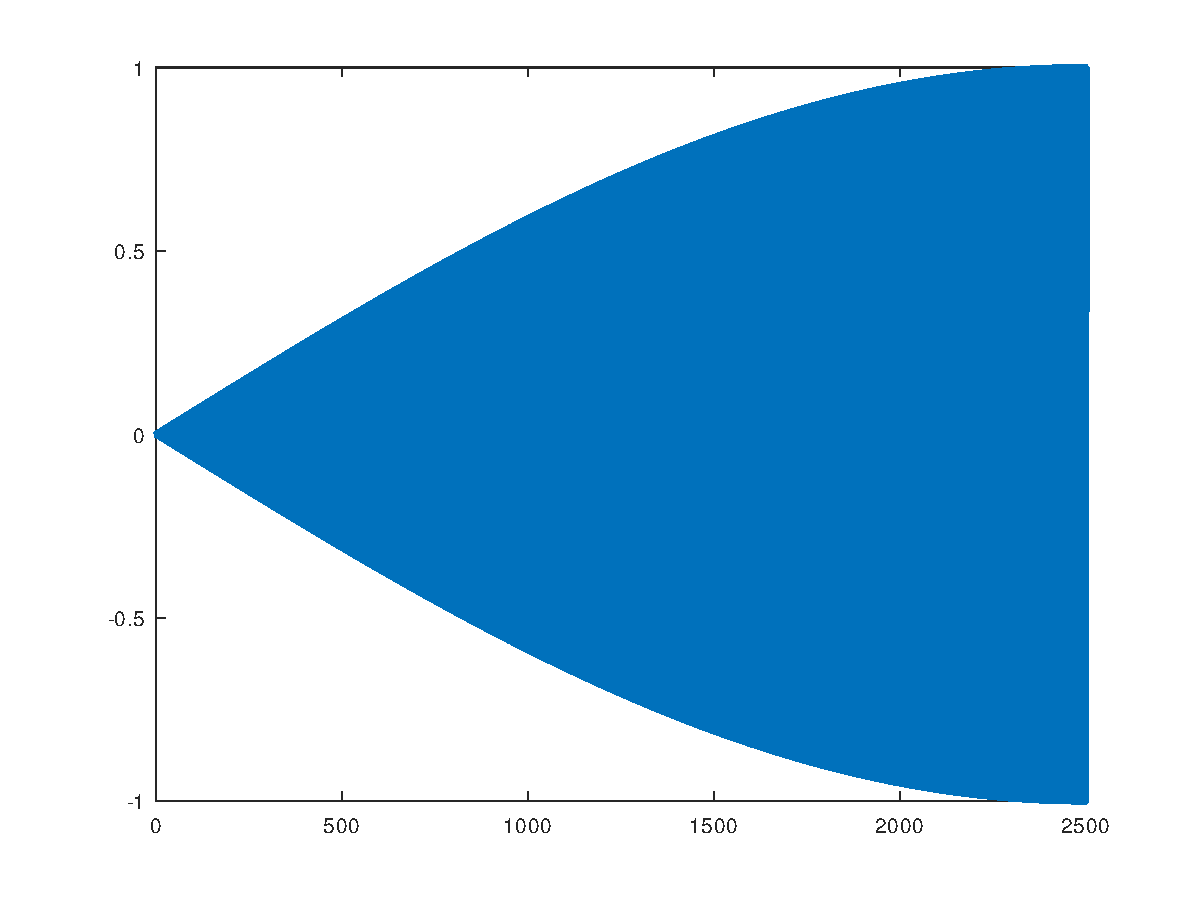
\includegraphics[
    width=\textwidth
    ]{papers/sgwt/images/dirac/dirac_fft_imag.pdf}
    \vspace{-0pt}
    \caption{Darstellung eines Dirac-Stoss $\delta(x)$ mit maximal Wert $1$. 
        \label{fig:sgwt:gft:dirac}}
    \end{minipage}
    ~
    \begin{minipage}[b]{0.49\textwidth}
    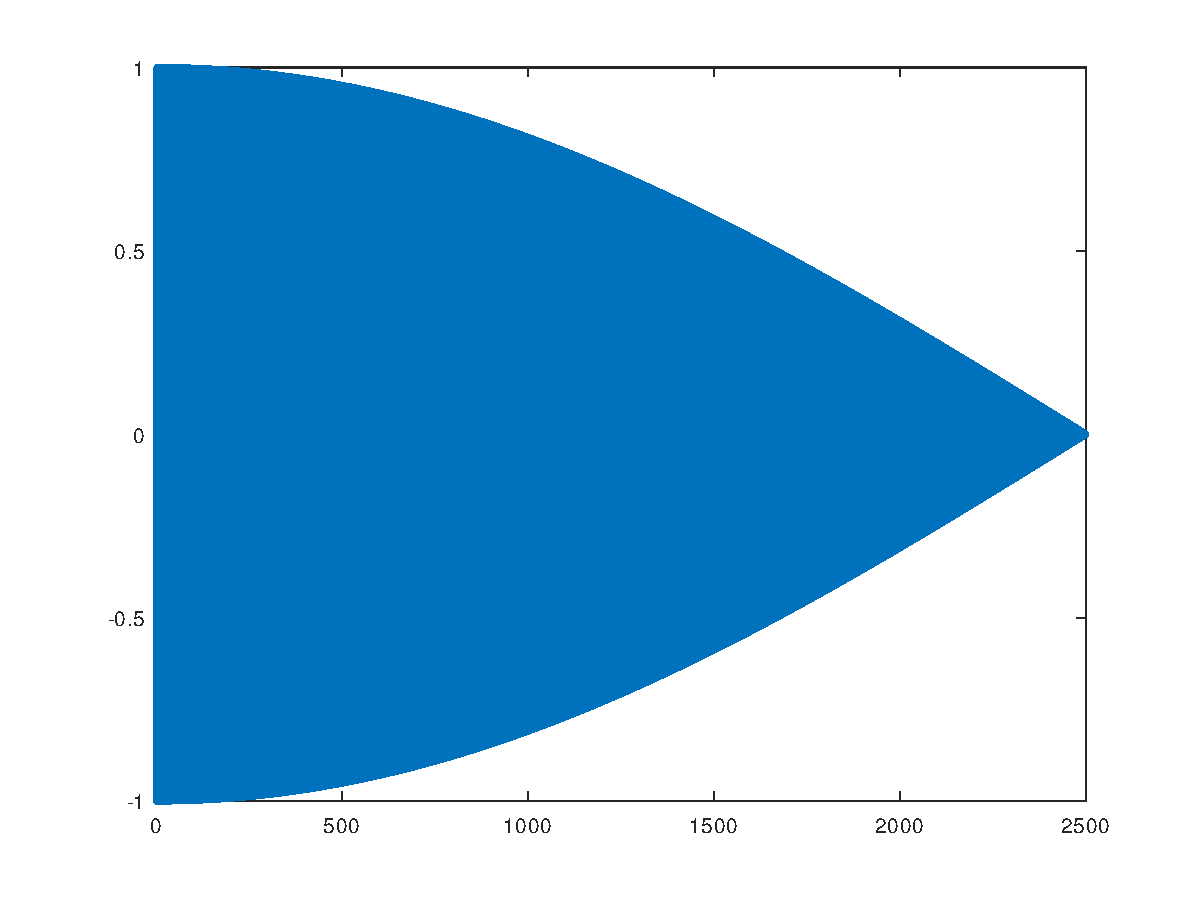
\includegraphics[
    width=\textwidth
    ]{papers/sgwt/images/dirac/dirac_fft_real.pdf}
    \vspace{-0pt}
    \caption{Fourier Transformation des Dirac-Stosses $\hat{\delta(x)}$ 
        aus~\cref{fig:sgwt:gft:dirac}.\label{fig:sgwt:gft:igft}}
    \end{minipage}
\end{figure}

\begin{figure}
    \centering
    \begin{minipage}[b]{0.49\textwidth}
    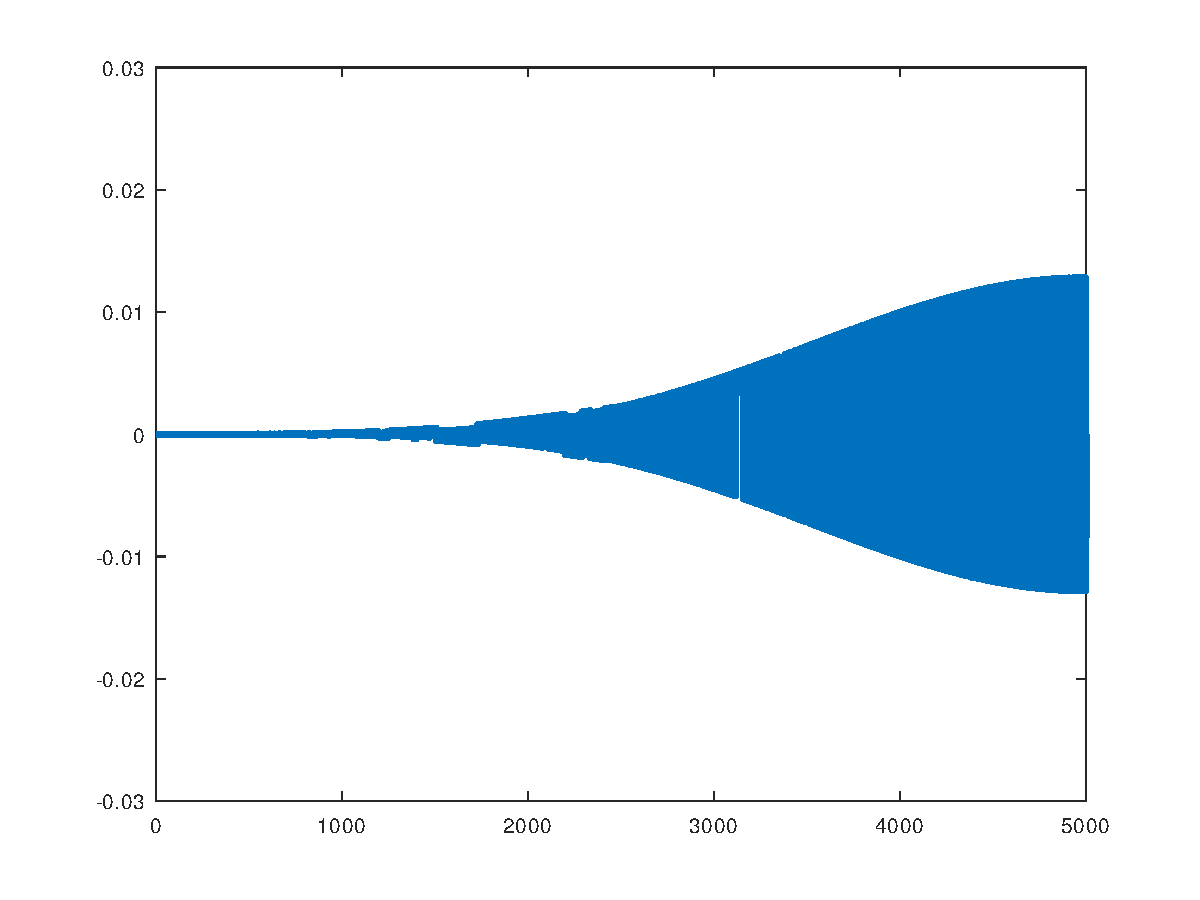
\includegraphics[
    width=\textwidth
    ]{papers/sgwt/images/dirac/dirac_gt1_gft.pdf}
    \vspace{-0pt}
    \caption{Darstellung eines Dirac-Stoss $\delta(x)$ mit maximal Wert $1$. 
        \label{fig:sgwt:gft:dirac}}
    \end{minipage}
    ~
    \begin{minipage}[b]{0.49\textwidth}
    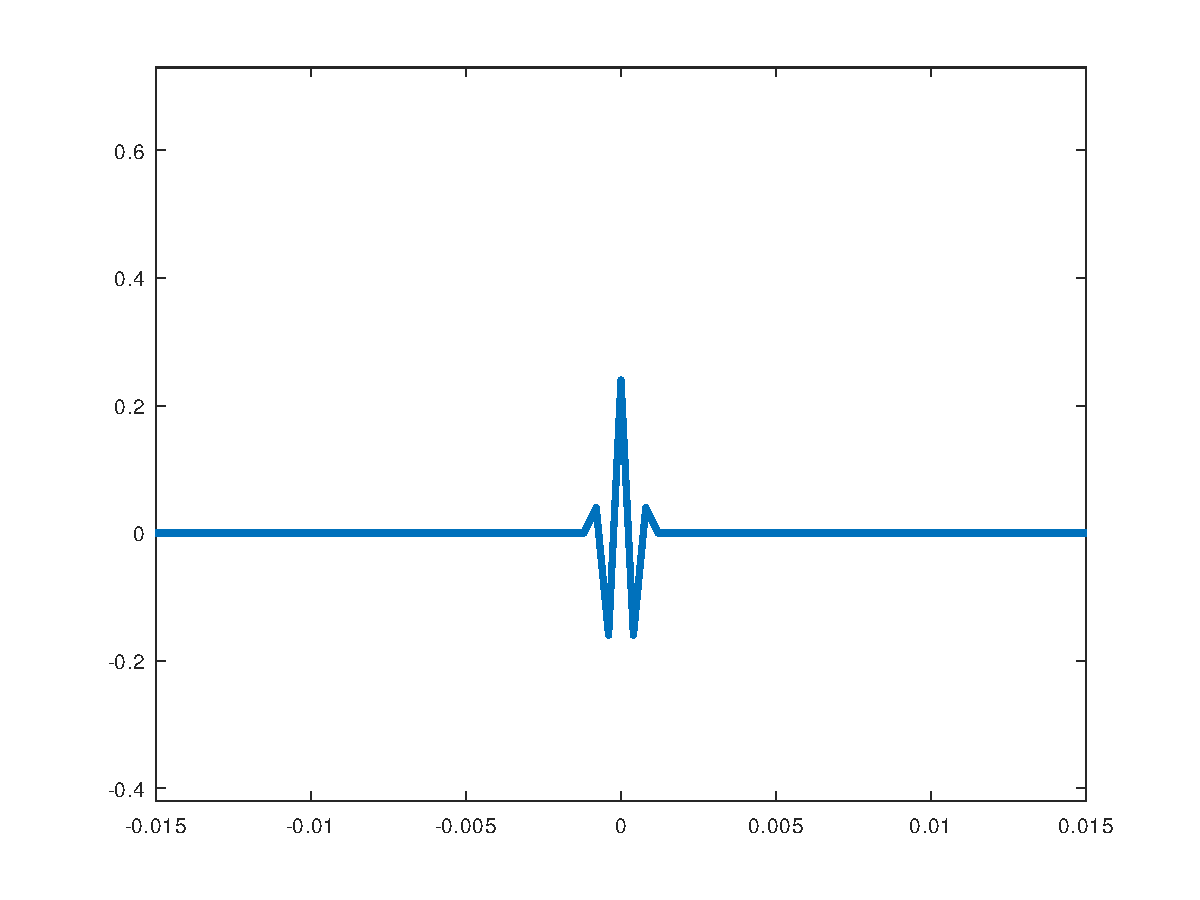
\includegraphics[
    width=\textwidth
    ]{papers/sgwt/images/dirac/dirac_gt1_igft.pdf}
    \vspace{-0pt}
    \caption{Fourier Transformation des Dirac-Stosses $\hat{\delta(x)}$ 
        aus~\cref{fig:sgwt:gft:dirac}.\label{fig:sgwt:gft:igft}}
    \end{minipage}
    ~
    \begin{minipage}[b]{0.49\textwidth}
    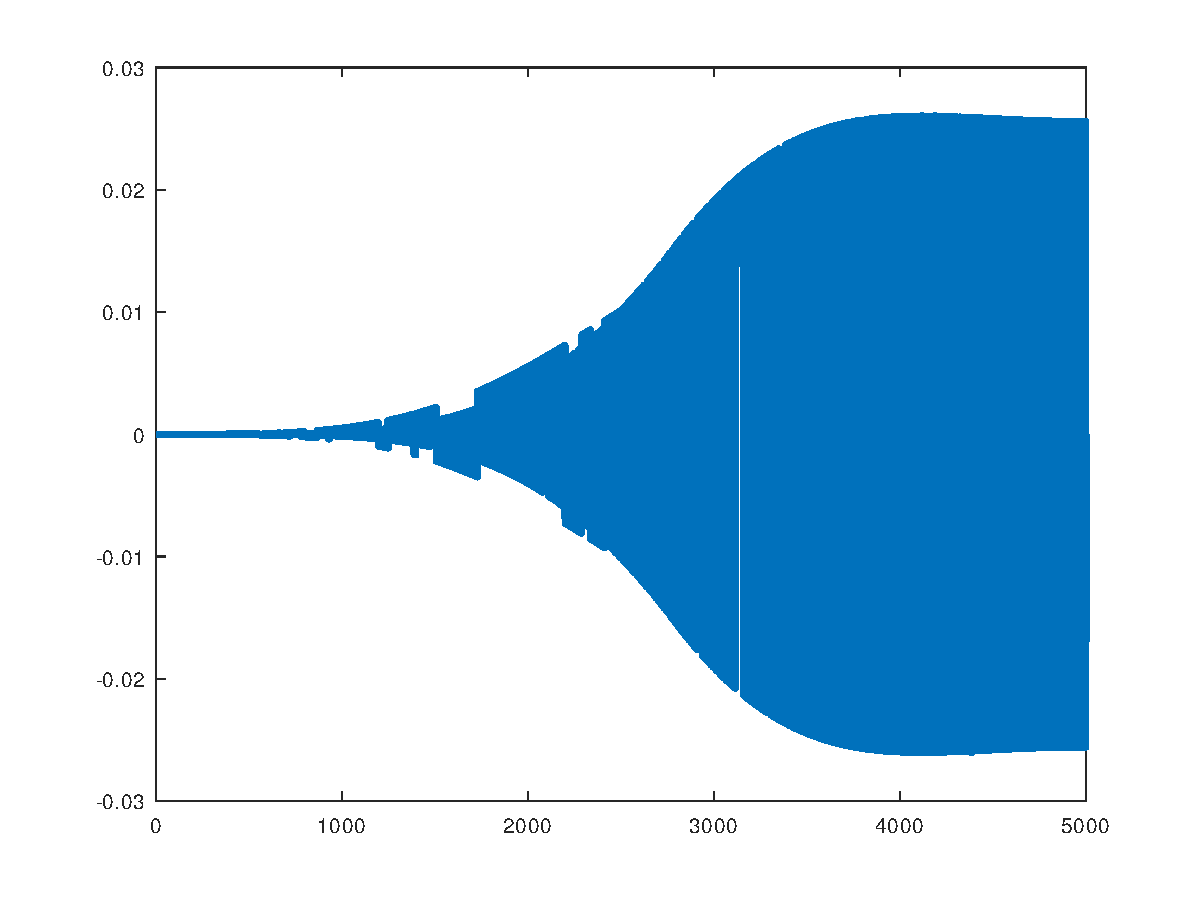
\includegraphics[
    width=\textwidth
    ]{papers/sgwt/images/dirac/dirac_gt2_gft.pdf}
    \vspace{-0pt}
    \caption{Fourier Transformation des Dirac-Stosses $\hat{\delta(x)}$ 
        aus~\cref{fig:sgwt:gft:dirac}.\label{fig:sgwt:gft:gft}}
    \end{minipage}
    ~
    \begin{minipage}[b]{0.49\textwidth}
    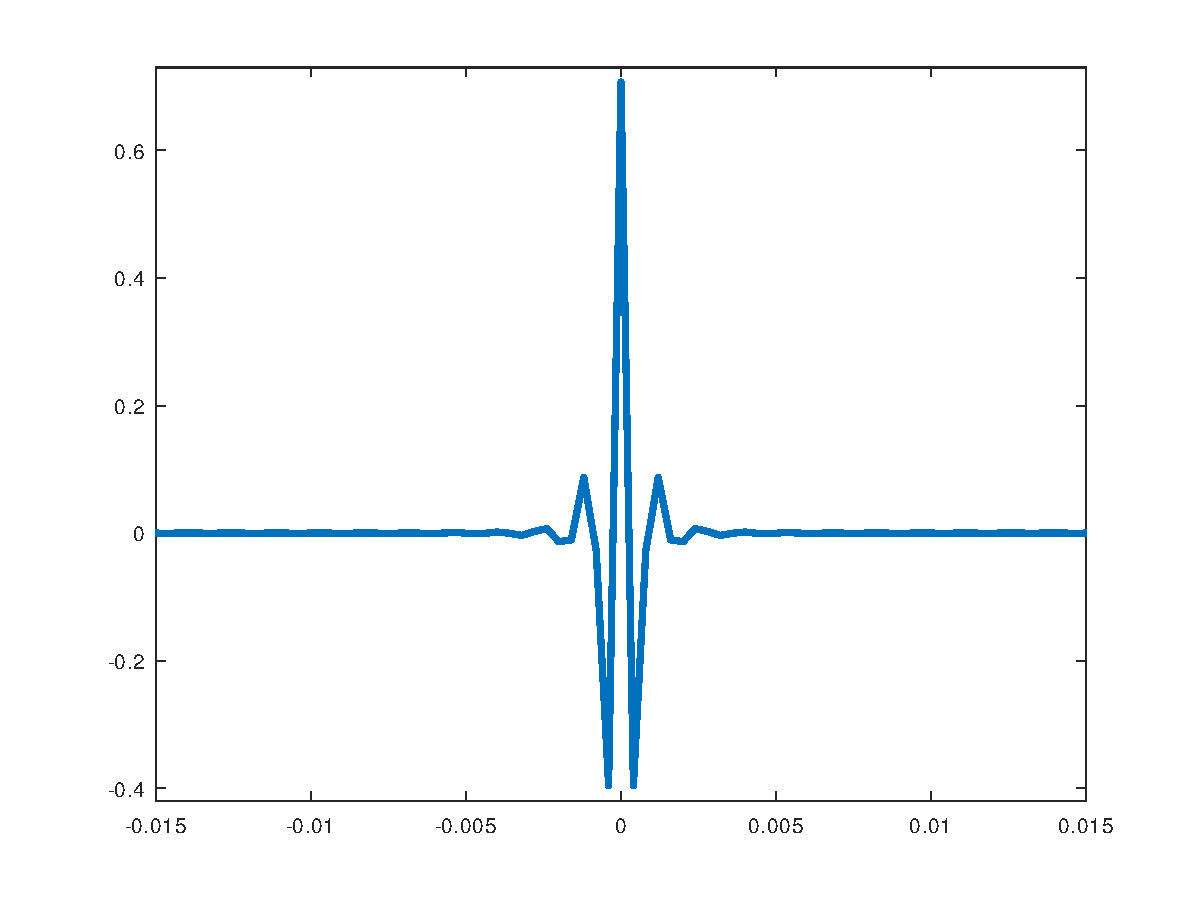
\includegraphics[
    width=\textwidth
    ]{papers/sgwt/images/dirac/dirac_gt2_igft.pdf}
    \vspace{-0pt}
    \caption{Fourier Transformation des Dirac-Stosses $\hat{\delta(x)}$ 
        aus~\cref{fig:sgwt:gft:dirac}.\label{fig:sgwt:gft:ggft}}
    \end{minipage}
    ~
    \begin{minipage}[b]{0.49\textwidth}
    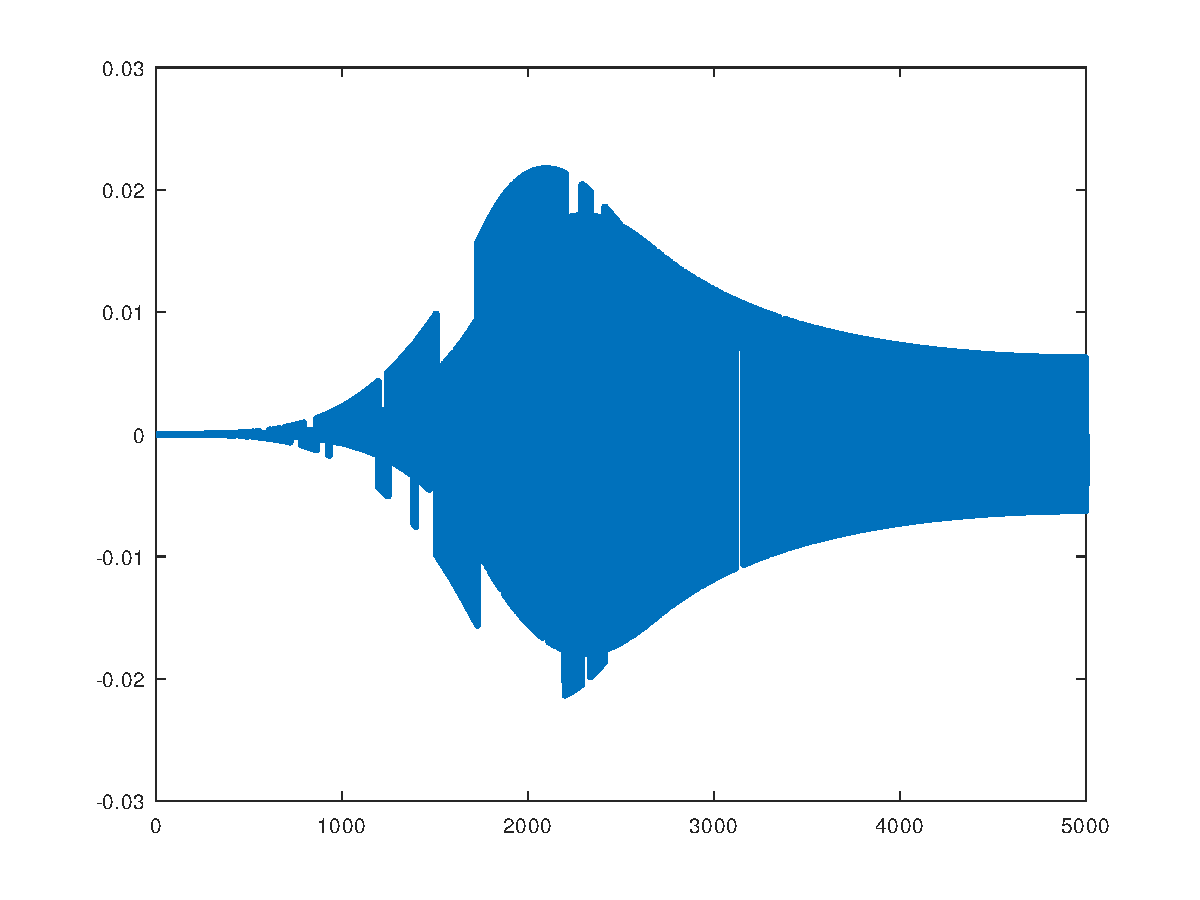
\includegraphics[
    width=\textwidth
    ]{papers/sgwt/images/dirac/dirac_gt3_gft.pdf}
    \vspace{-0pt}
    \caption{Fourier Transformation des Dirac-Stosses $\hat{\delta(x)}$ 
        aus~\cref{fig:sgwt:gft:dirac}.\label{fig:sgwt:gft:ggft}}
    \end{minipage}
    ~
    \begin{minipage}[b]{0.49\textwidth}
    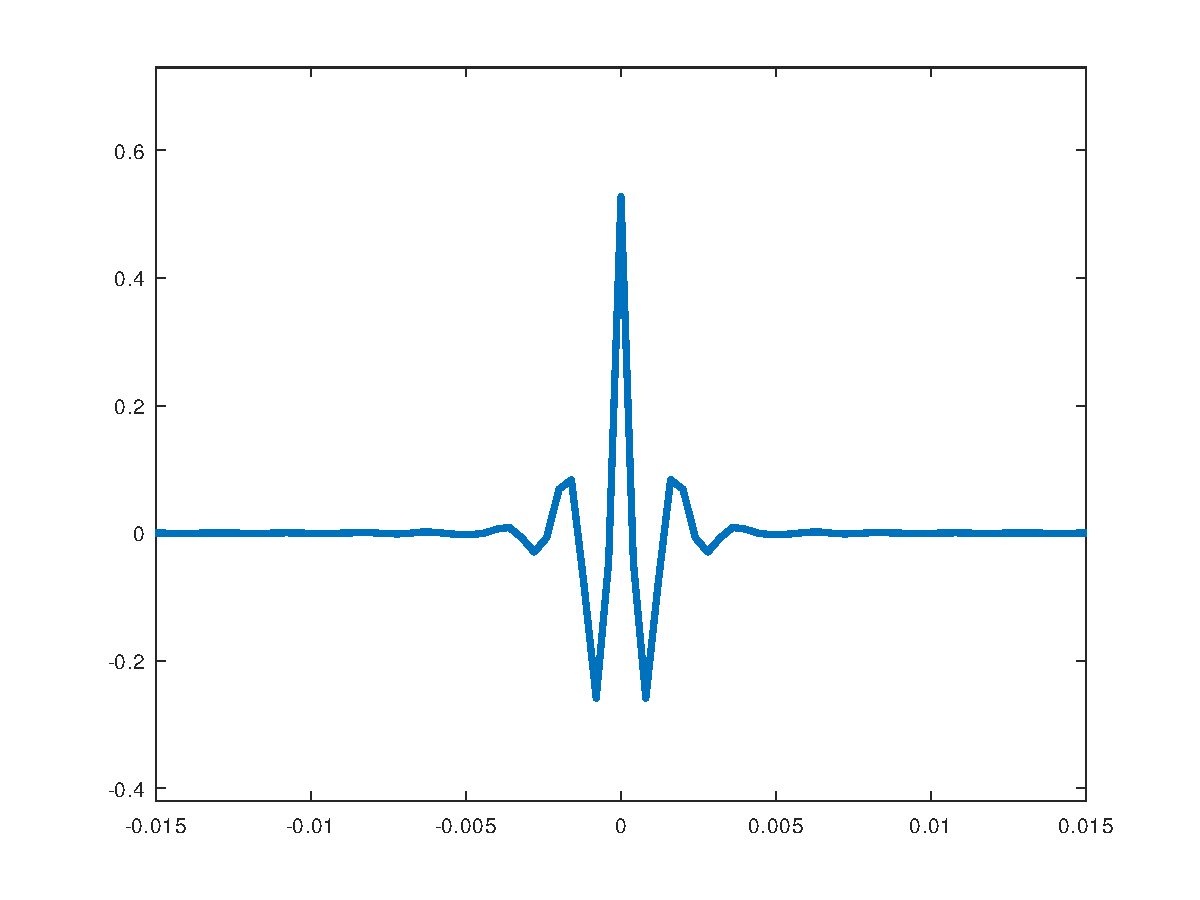
\includegraphics[
    width=\textwidth
    ]{papers/sgwt/images/dirac/dirac_gt3_igft.pdf}
    \vspace{-0pt}
    \caption{Fourier Transformation des Dirac-Stosses $\hat{\delta(x)}$ 
        aus~\cref{fig:sgwt:gft:dirac}.\label{fig:sgwt:gft:ggft}}
    \end{minipage}
\end{figure}



\begin{figure}
    \centering
    \begin{minipage}[b]{0.49\textwidth}
    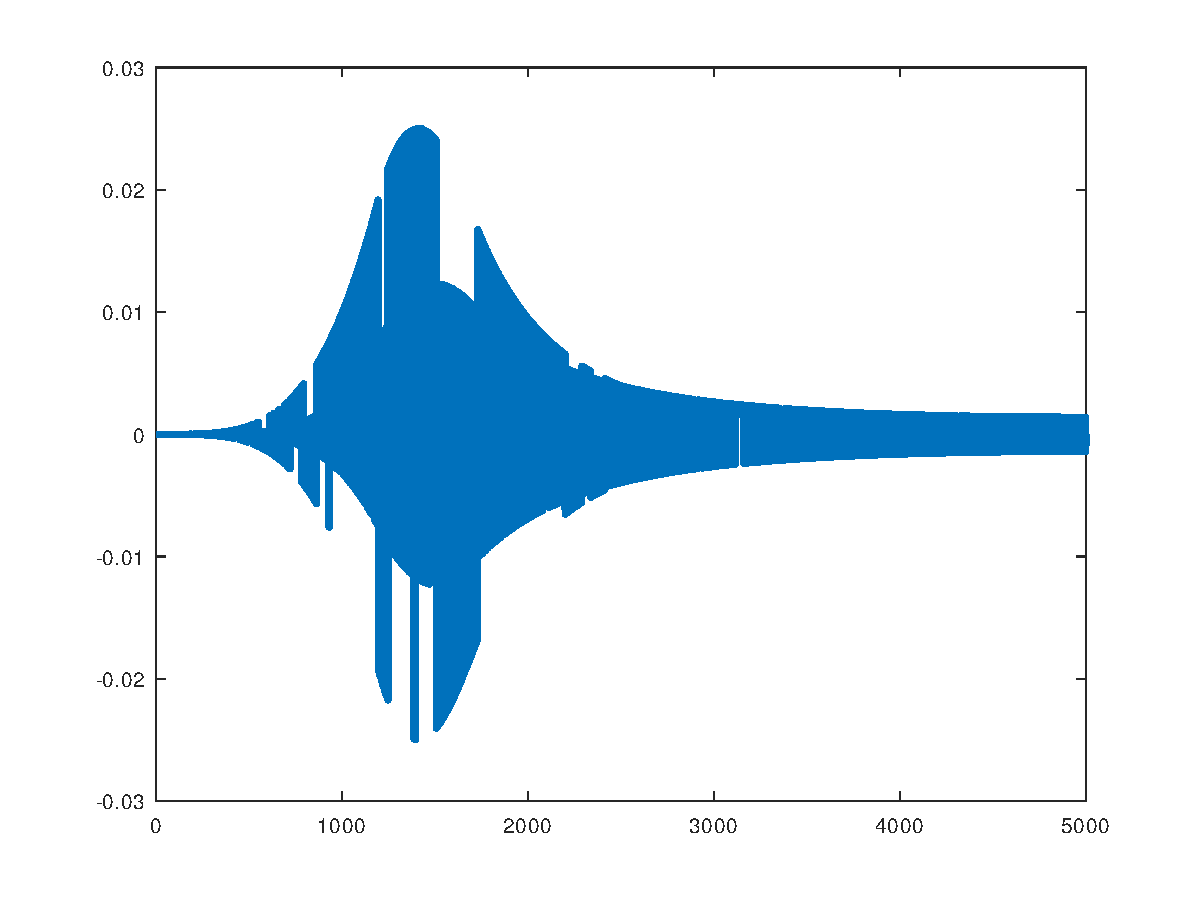
\includegraphics[
    width=\textwidth
    ]{papers/sgwt/images/dirac/dirac_gt4_gft.pdf}
    \vspace{-0pt}
    \caption{Darstellung eines Dirac-Stoss $\delta(x)$ mit maximal Wert $1$. 
        \label{fig:sgwt:gft:dirac}}
    \end{minipage}
    ~
    \begin{minipage}[b]{0.49\textwidth}
    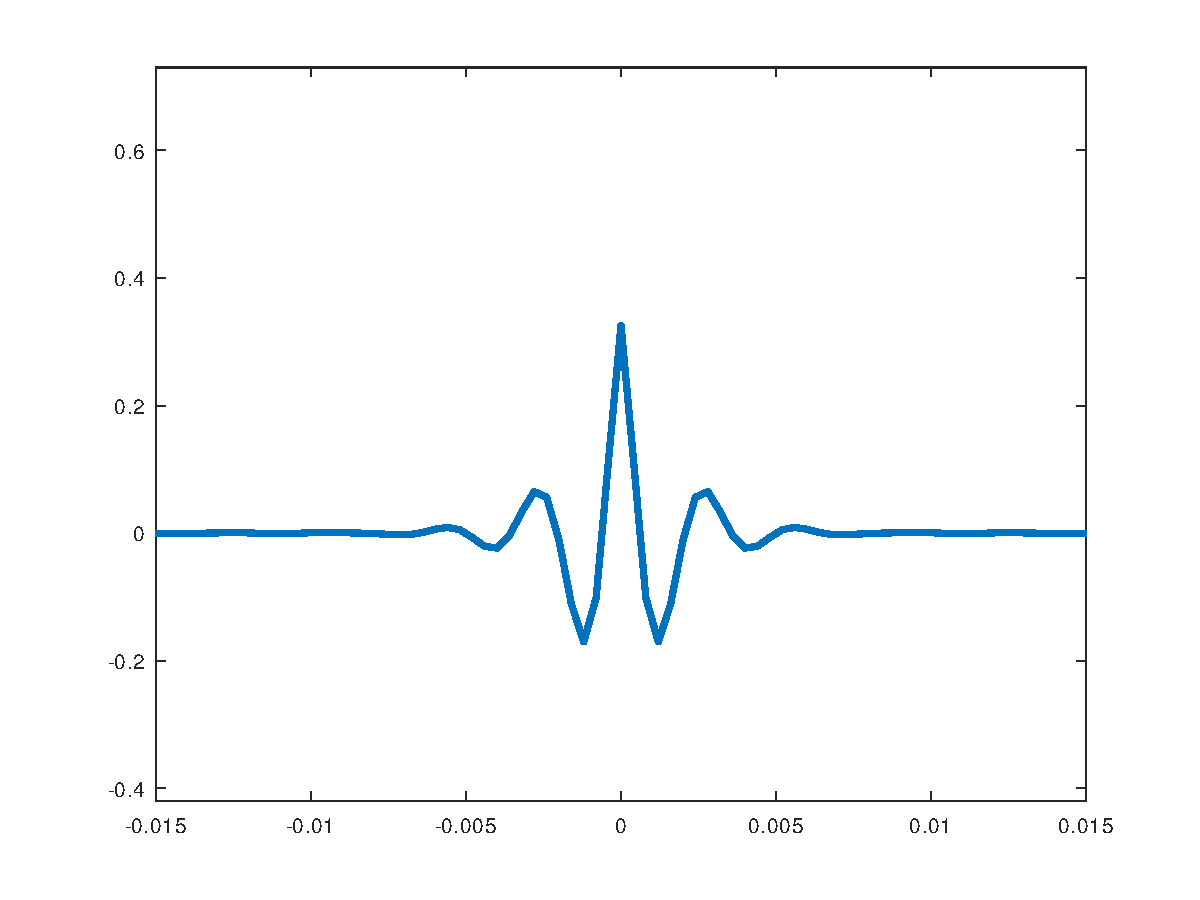
\includegraphics[
    width=\textwidth
    ]{papers/sgwt/images/dirac/dirac_gt4_igft.pdf}
    \vspace{-0pt}
    \caption{Fourier Transformation des Dirac-Stosses $\hat{\delta(x)}$ 
        aus~\cref{fig:sgwt:gft:dirac}.\label{fig:sgwt:gft:igft}}
    \end{minipage}
    ~
    \begin{minipage}[b]{0.49\textwidth}
    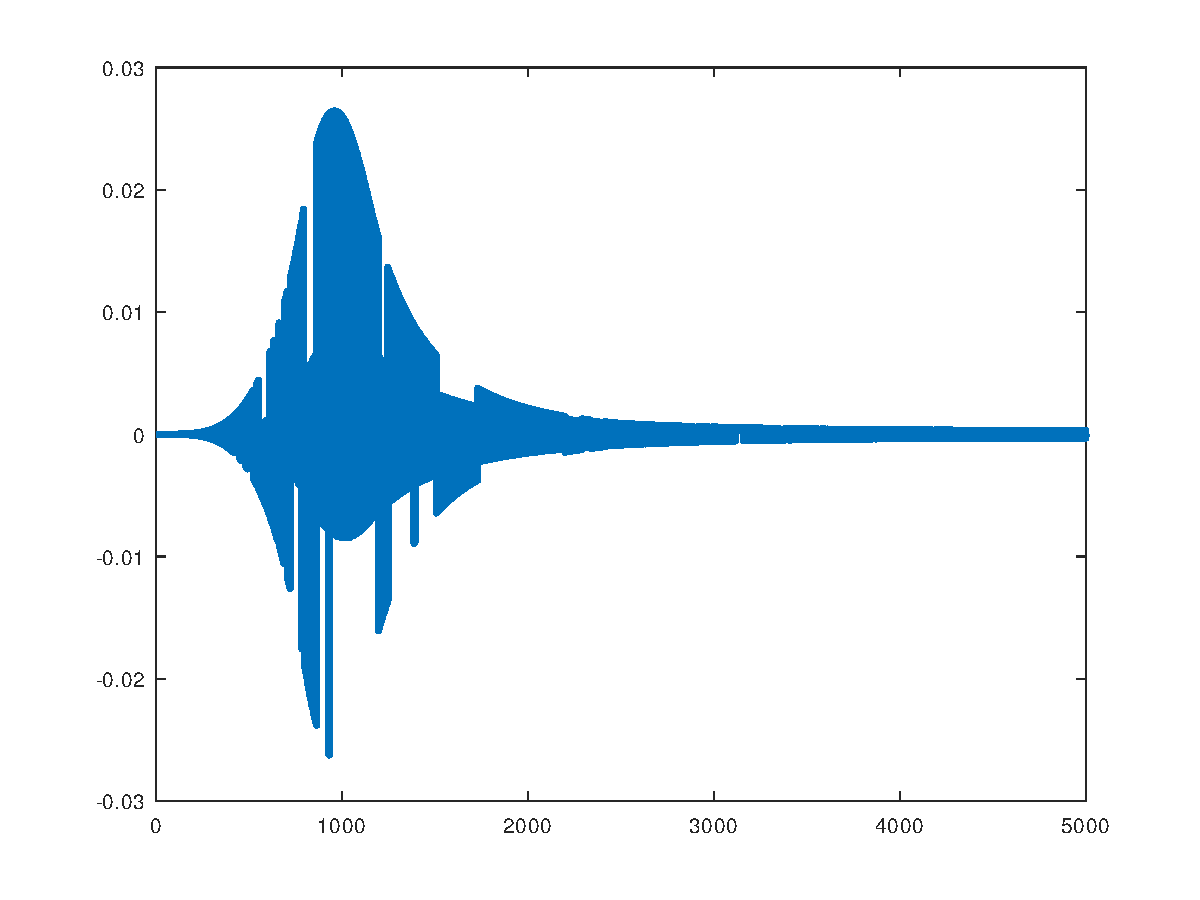
\includegraphics[
    width=\textwidth
    ]{papers/sgwt/images/dirac/dirac_gt5_gft.pdf}
    \vspace{-0pt}
    \caption{Fourier Transformation des Dirac-Stosses $\hat{\delta(x)}$ 
        aus~\cref{fig:sgwt:gft:dirac}.\label{fig:sgwt:gft:gft}}
    \end{minipage}
    ~
    \begin{minipage}[b]{0.49\textwidth}
    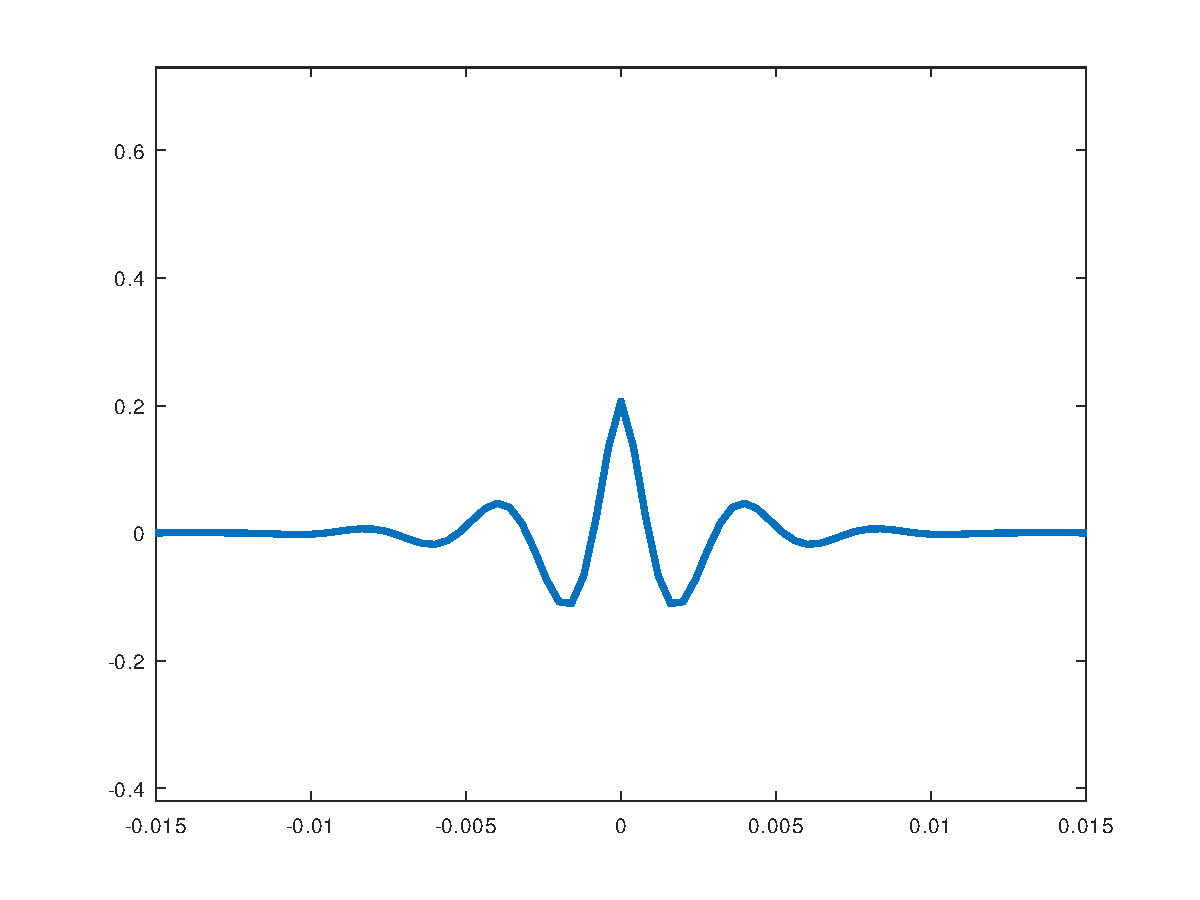
\includegraphics[
    width=\textwidth
    ]{papers/sgwt/images/dirac/dirac_gt5_igft.pdf}
    \vspace{-0pt}
    \caption{Fourier Transformation des Dirac-Stosses $\hat{\delta(x)}$ 
        aus~\cref{fig:sgwt:gft:dirac}.\label{fig:sgwt:gft:ggft}}
    \end{minipage}
    ~
    \begin{minipage}[b]{0.49\textwidth}
    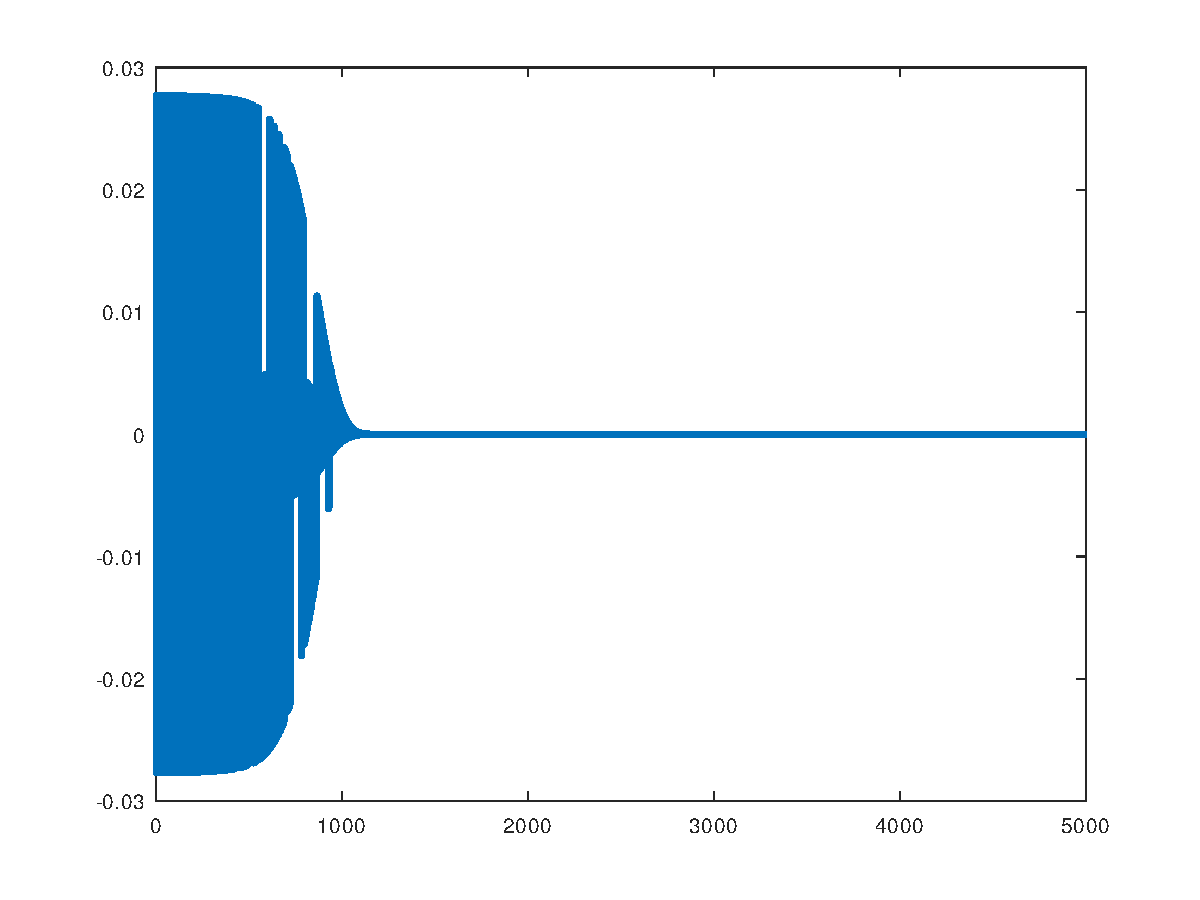
\includegraphics[
    width=\textwidth
    ]{papers/sgwt/images/dirac/dirac_h_gft.pdf}
    \vspace{-0pt}
    \caption{Fourier Transformation des Dirac-Stosses $\hat{\delta(x)}$ 
        aus~\cref{fig:sgwt:gft:dirac}.\label{fig:sgwt:gft:ggft}}
    \end{minipage}
    ~
    \begin{minipage}[b]{0.49\textwidth}
    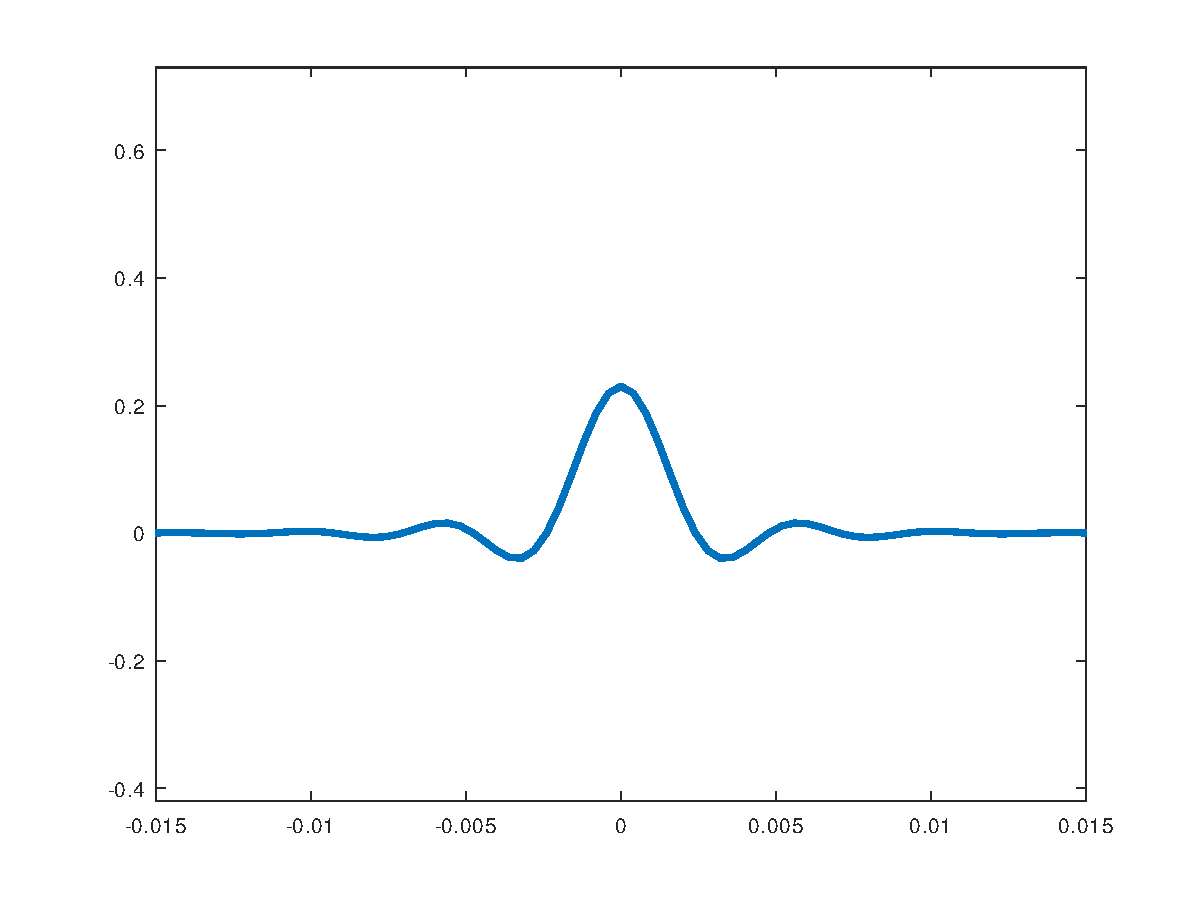
\includegraphics[
    width=\textwidth
    ]{papers/sgwt/images/dirac/dirac_h_igft.pdf}
    \vspace{-0pt}
    \caption{Fourier Transformation des Dirac-Stosses $\hat{\delta(x)}$ 
        aus~\cref{fig:sgwt:gft:dirac}.\label{fig:sgwt:gft:ggft}}
    \end{minipage}
\end{figure}

\begin{figure}
    \centering
    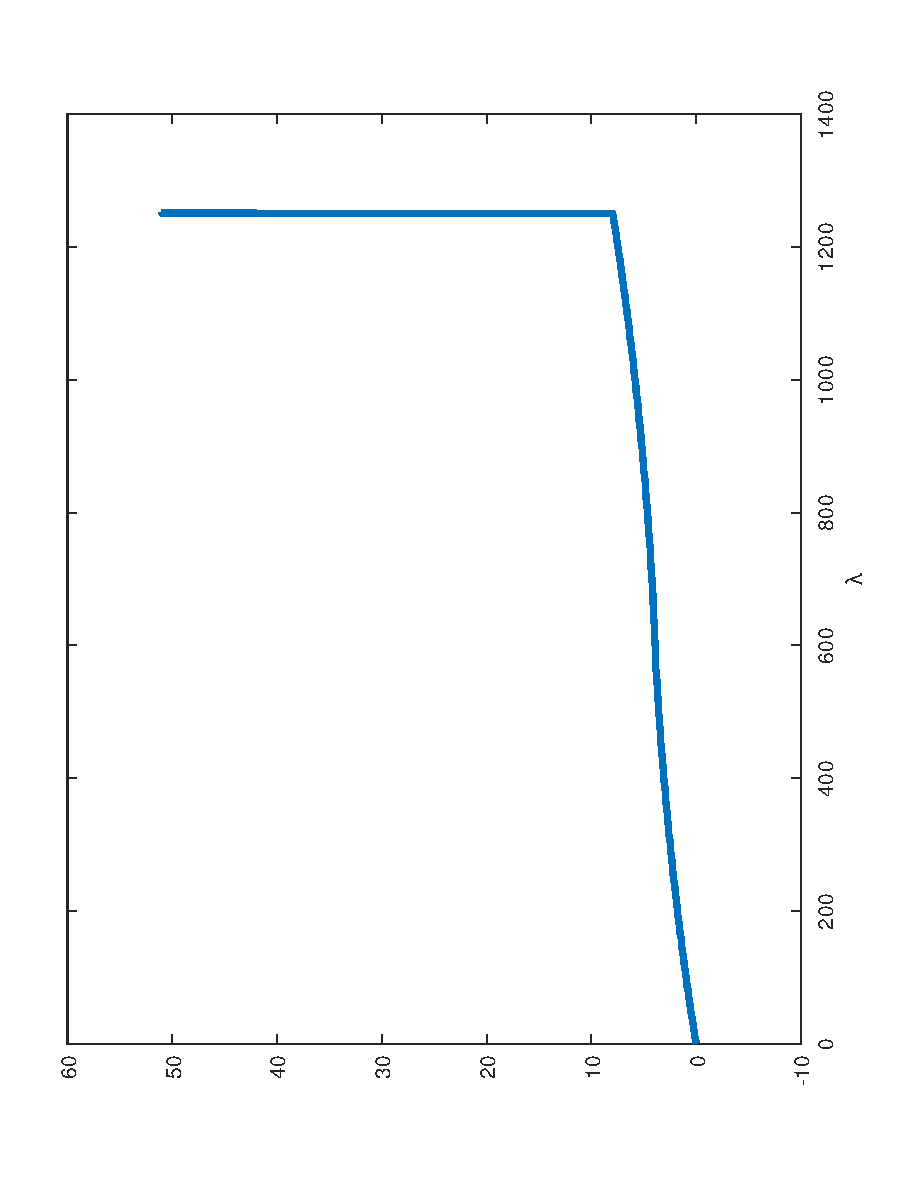
\includegraphics[
    angle=-90,
    origin=c,
    scale=0.6
    ]{papers/sgwt/images/wavelets/lambda.pdf}
    \vspace{-50pt}
    \caption{Eigenwerte $\lambda$ eines Kugelgraphen mit 1252 Knoten. 
    \label{fig:sgwt:wavelets:sphere:lambda}}
\end{figure}

\begin{figure}
    \begin{minipage}[b]{0.49\textwidth}
        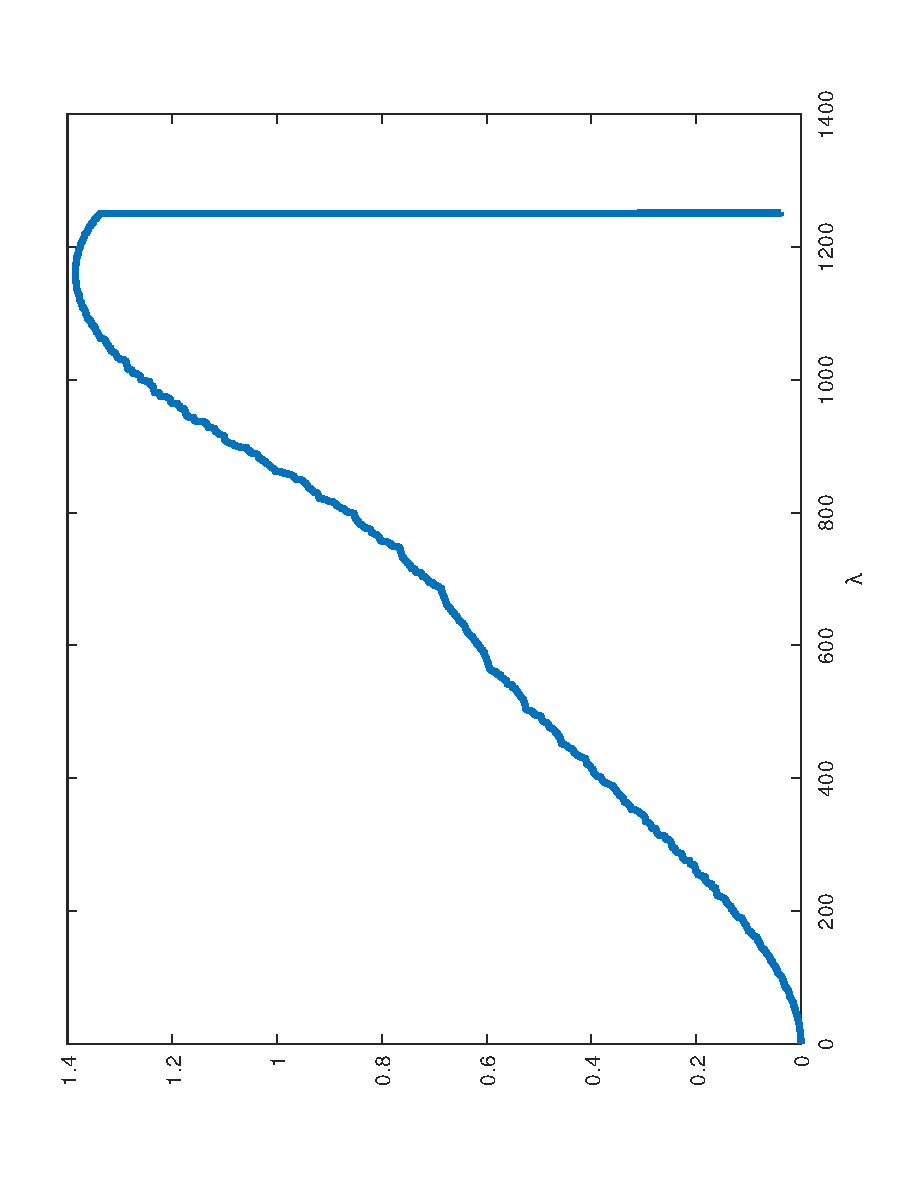
\includegraphics[
        angle=-90,
        origin=c,
        width=\textwidth]{papers/sgwt/images/wavelets/gt1.pdf}
        \vspace{-45pt}
        \caption{Die Kernelfunktion $g(t_1\lambda)$ eines Kugelgraphen mit 1252 
        Knoten und $t_1 = 0.2$.}
        \label{fig:sgwt:wavelets:sphere:gt1}
    \end{minipage}
    ~
    \begin{minipage}[b]{0.49\textwidth}
        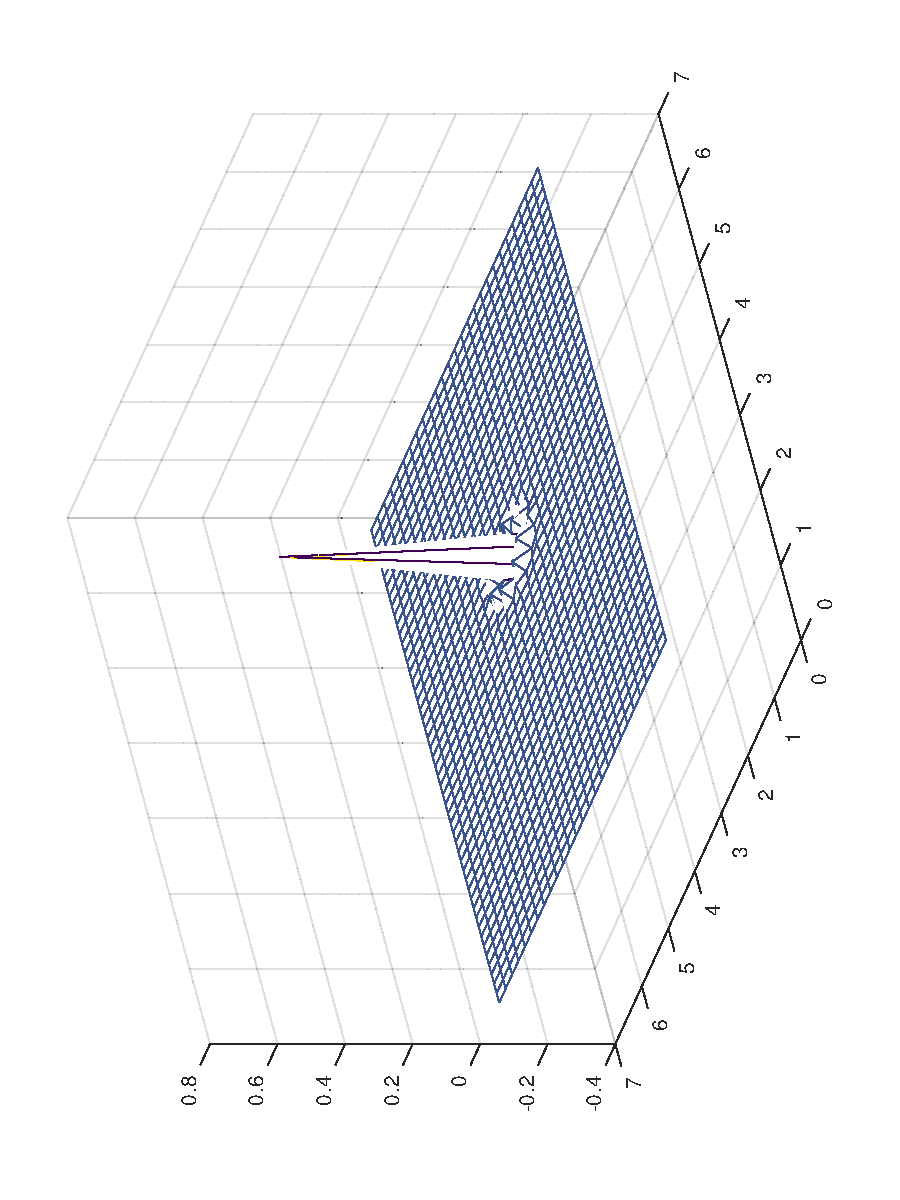
\includegraphics[
        angle=-90,
        origin=c,
        width=\textwidth]{papers/sgwt/images/wavelets/psi_t1_50_25_630_flat.pdf}
        \vspace{-45pt}
        \caption{$\psi_1(v_{630})$-Wavelet eines Kugelgraphen mit 1252 Knoten.}
        \label{fig:sgwt:wavelets:sphere:psi1:flat}
    \end{minipage}
    ~
    \begin{minipage}[b]{\textwidth}
        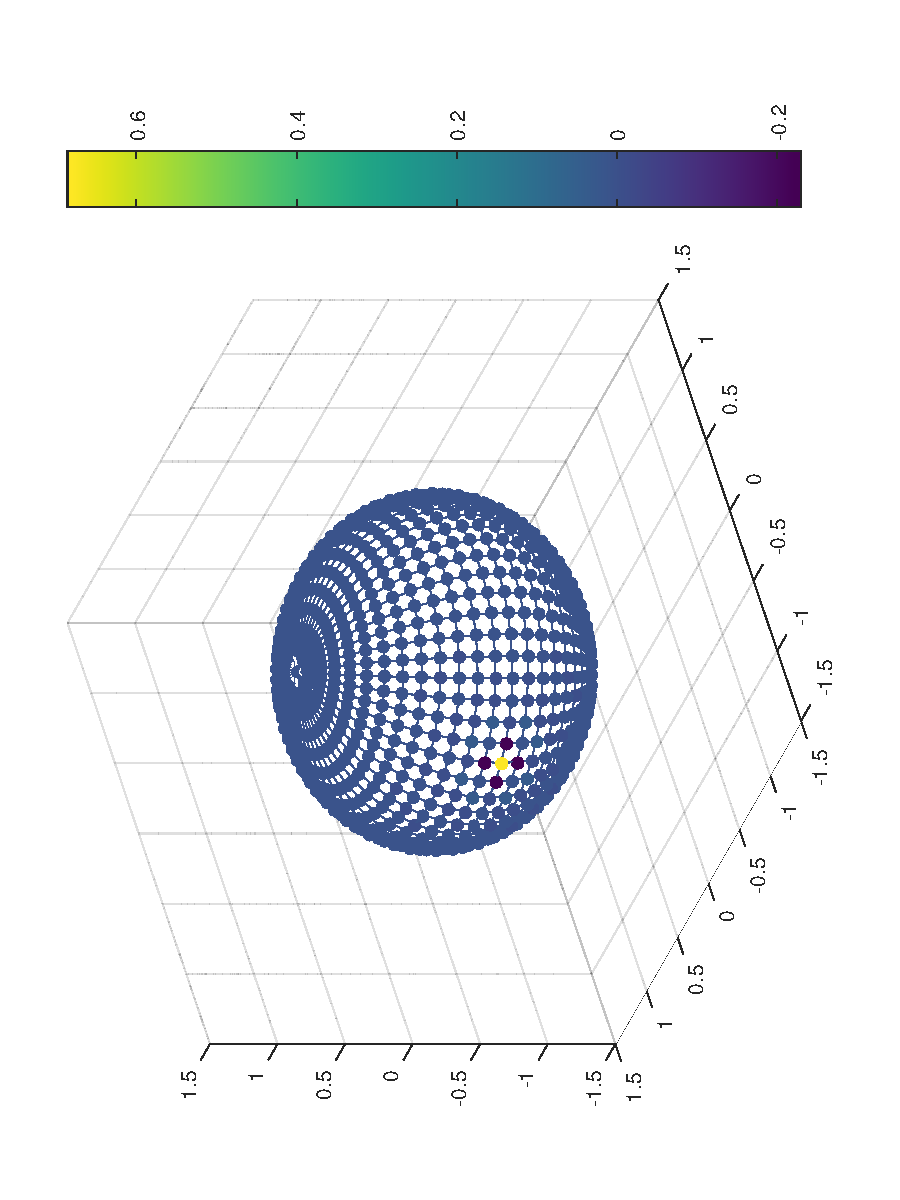
\includegraphics[
        angle=-90,
        origin=c,
        width=\textwidth]{papers/sgwt/images/wavelets/psi_t1_50_25_630.pdf}
        \vspace{-45pt}
        \caption{$\psi_1(v_{630})$-Wavelet eines Kugelgraphen mit 1252 Knoten 
        und $t = 0.42295$.}
        \label{fig:sgwt:wavelets:sphere:psi1}
    \end{minipage}
\end{figure}

\begin{figure}
    \begin{minipage}[b]{0.49\textwidth}
        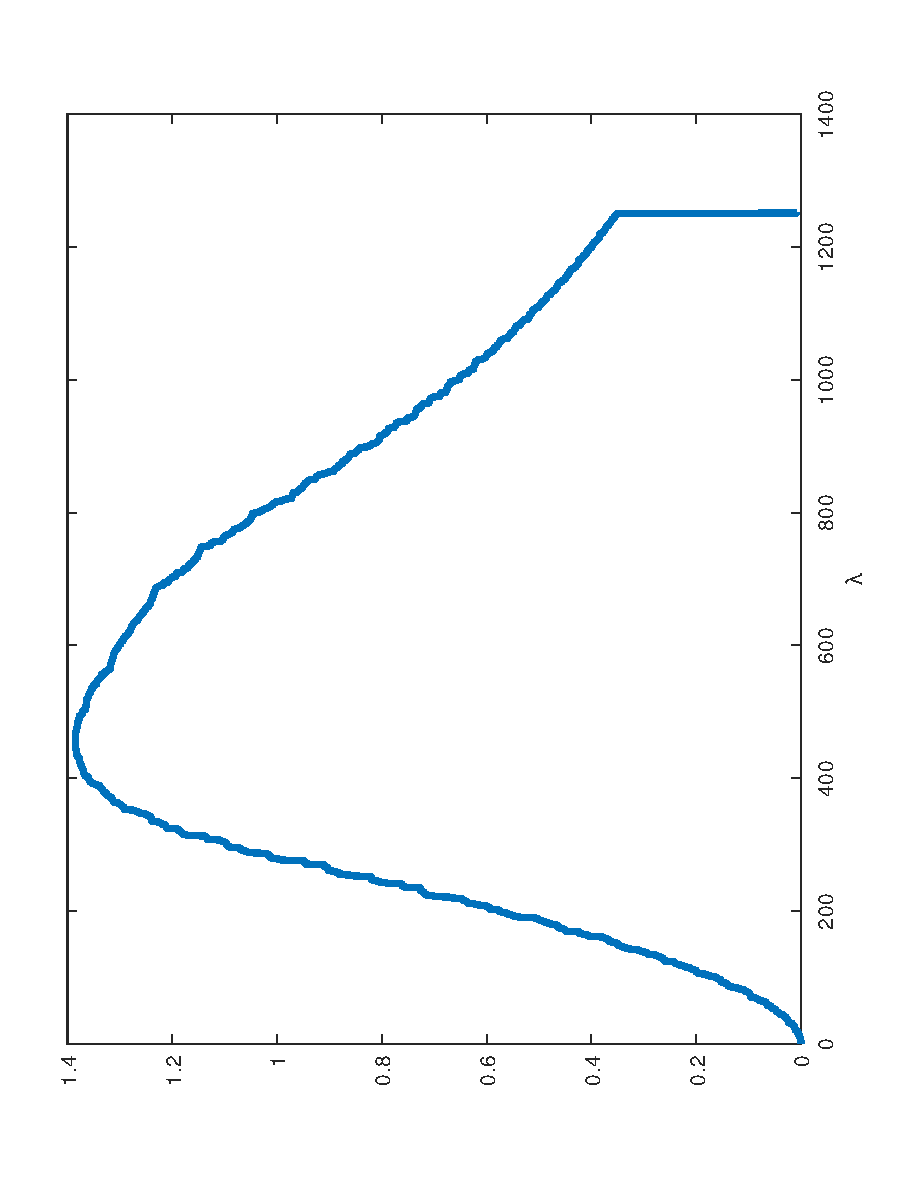
\includegraphics[
        angle=-90,
        origin=c,
        width=\textwidth]{papers/sgwt/images/wavelets/gt2.pdf}
        \vspace{-45pt}
        \caption{Die Kernelfunktion $g(t_2\lambda)$ eines Kugelgraphen mit 1252 
            Knoten und $t_2 = 0.42295$.}
        \label{fig:sgwt:wavelets:sphere:gt2}
    \end{minipage}
    ~
    \begin{minipage}[b]{0.49\textwidth}
        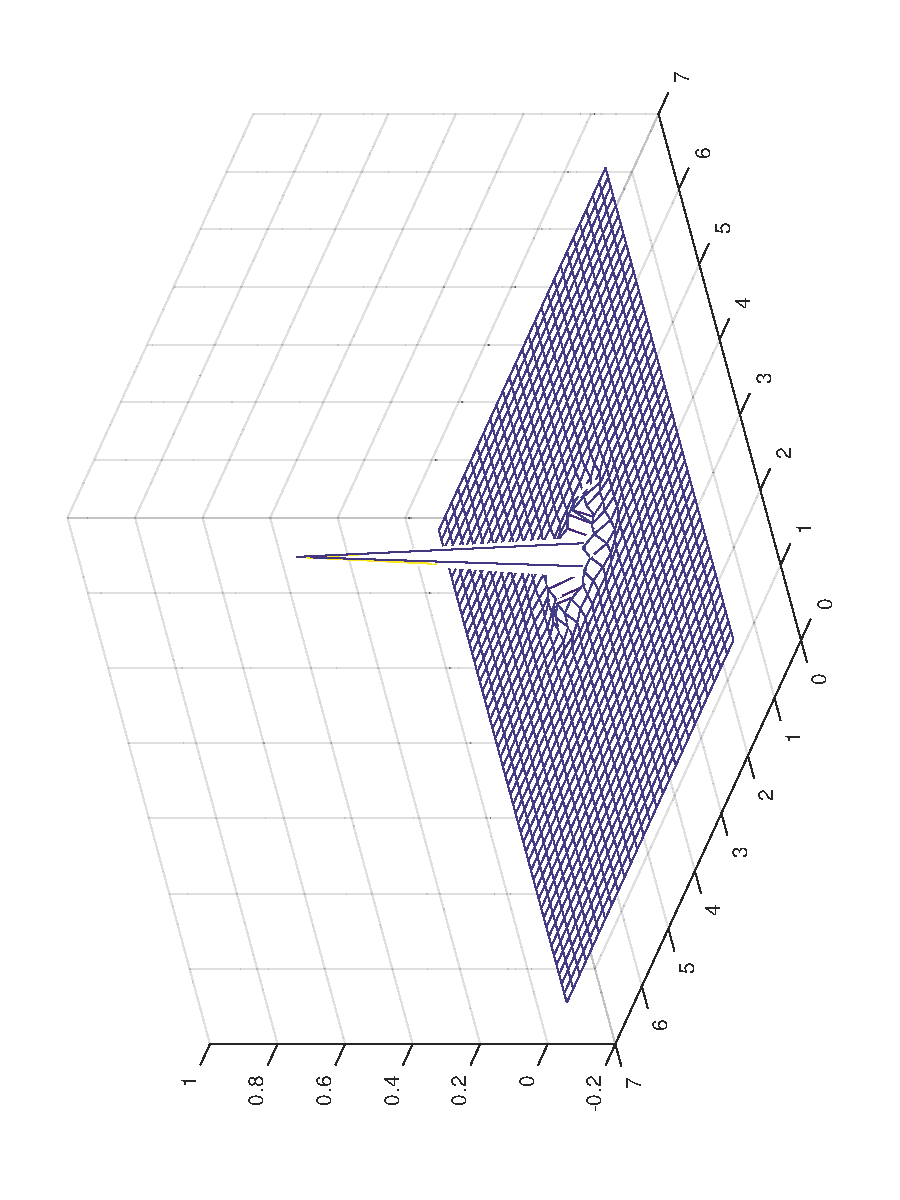
\includegraphics[
        angle=-90,
        origin=c,
        width=\textwidth]{papers/sgwt/images/wavelets/psi_t2_50_25_630_flat.pdf}
        \vspace{-45pt}
        \caption{$\psi_2(v_{630})$-Wavelet eines Kugelgraphen mit 1252 Knoten.}
        \label{fig:sgwt:wavelets:sphere:psi2:flat}
    \end{minipage}
    ~
    \begin{minipage}[b]{\textwidth}
        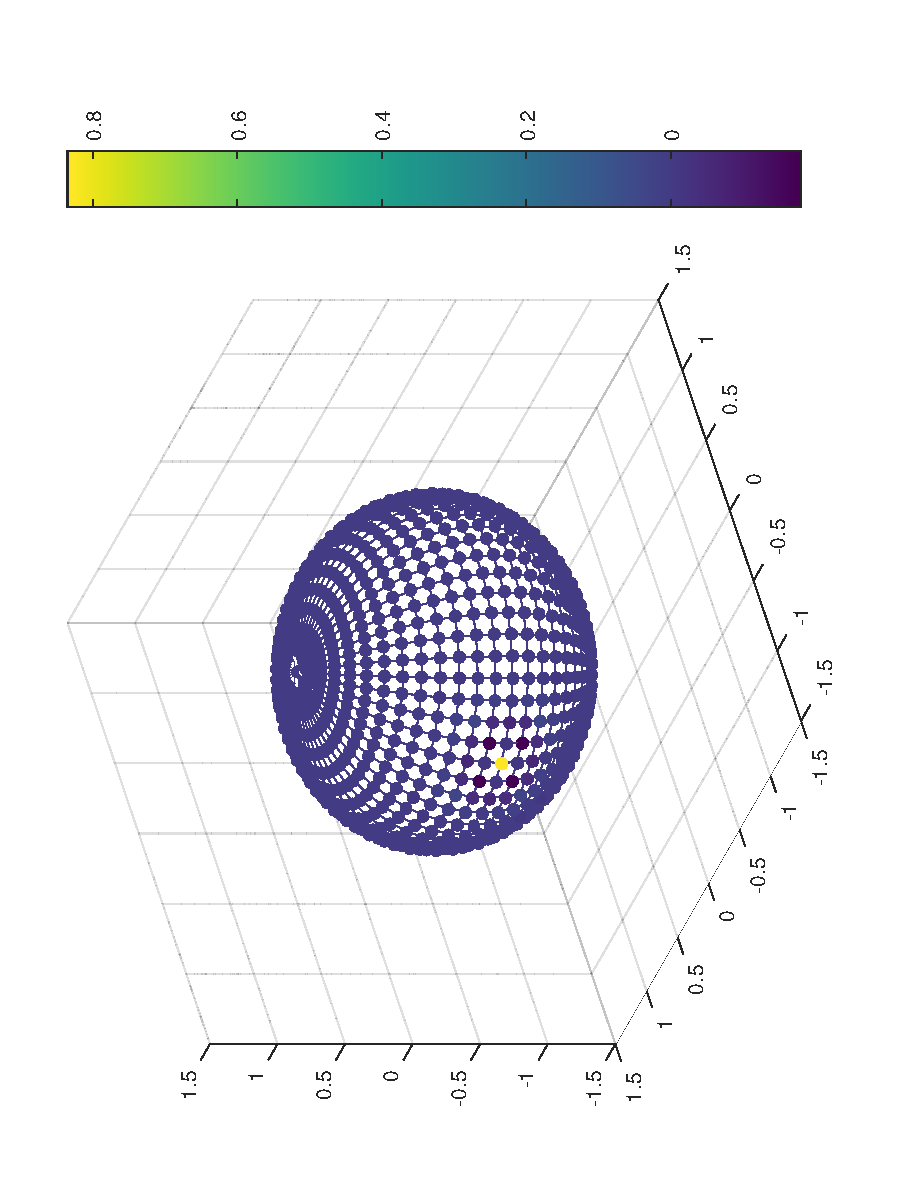
\includegraphics[
        angle=-90,
        origin=c,
        width=\textwidth]{papers/sgwt/images/wavelets/psi_t2_50_25_630.pdf}
        \vspace{-45pt}
        \caption{$\psi_2(v_{630})$-Wavelet eines Kugelgraphen mit 1252 Knoten.}
        \label{fig:sgwt:wavelets:sphere:psi2}
    \end{minipage}
\end{figure}

\begin{figure}
    \begin{minipage}[b]{0.49\textwidth}
        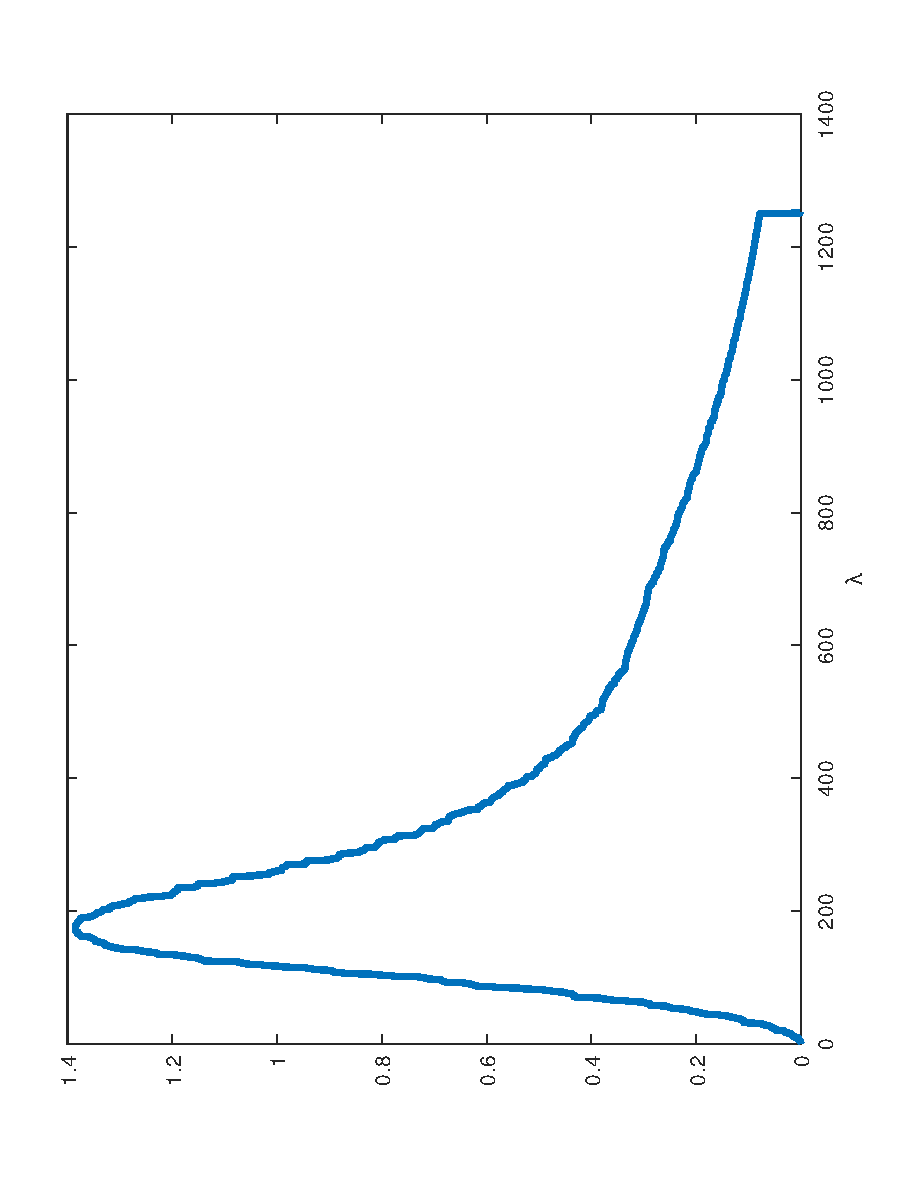
\includegraphics[
        angle=-90,
        origin=c,
        width=\textwidth]{papers/sgwt/images/wavelets/gt3.pdf}
        \vspace{-45pt}
        \caption{Die Kernelfunktion $g(t_3\lambda)$ eines Kugelgraphen mit 1252 
            Knoten und $t_3 = 0.89443$.}
        \label{fig:sgwt:wavelets:sphere:gt3}
    \end{minipage}
    ~
    \begin{minipage}[b]{0.49\textwidth}
        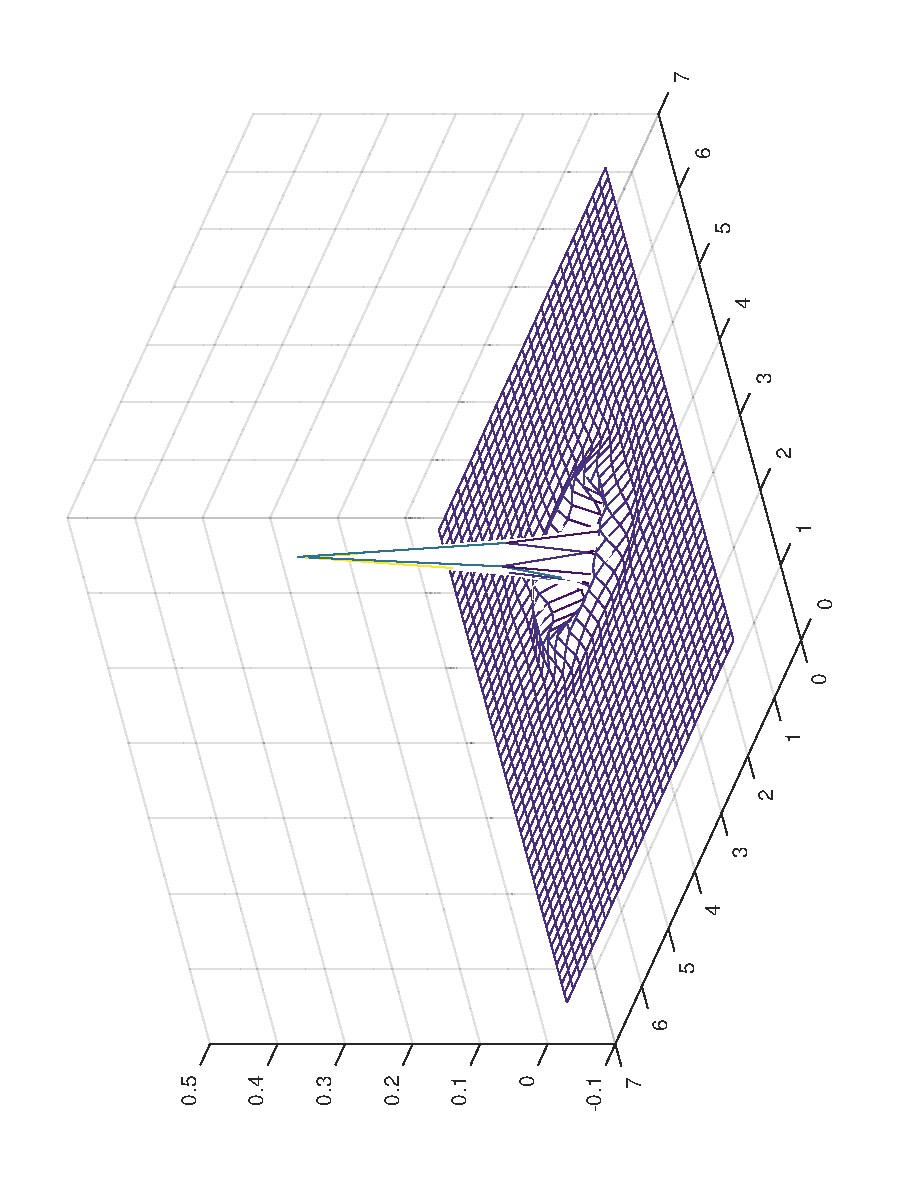
\includegraphics[
        angle=-90,
        origin=c,
        width=\textwidth]{papers/sgwt/images/wavelets/psi_t3_50_25_630_flat.pdf}
        \vspace{-45pt}
        \caption{$\psi_3(v_{630})$-Wavelet eines Kugelgraphen mit 1252 Knoten.}
        \label{fig:sgwt:wavelets:sphere:psi3:flat}
    \end{minipage}
    ~
    \begin{minipage}[b]{\textwidth}
        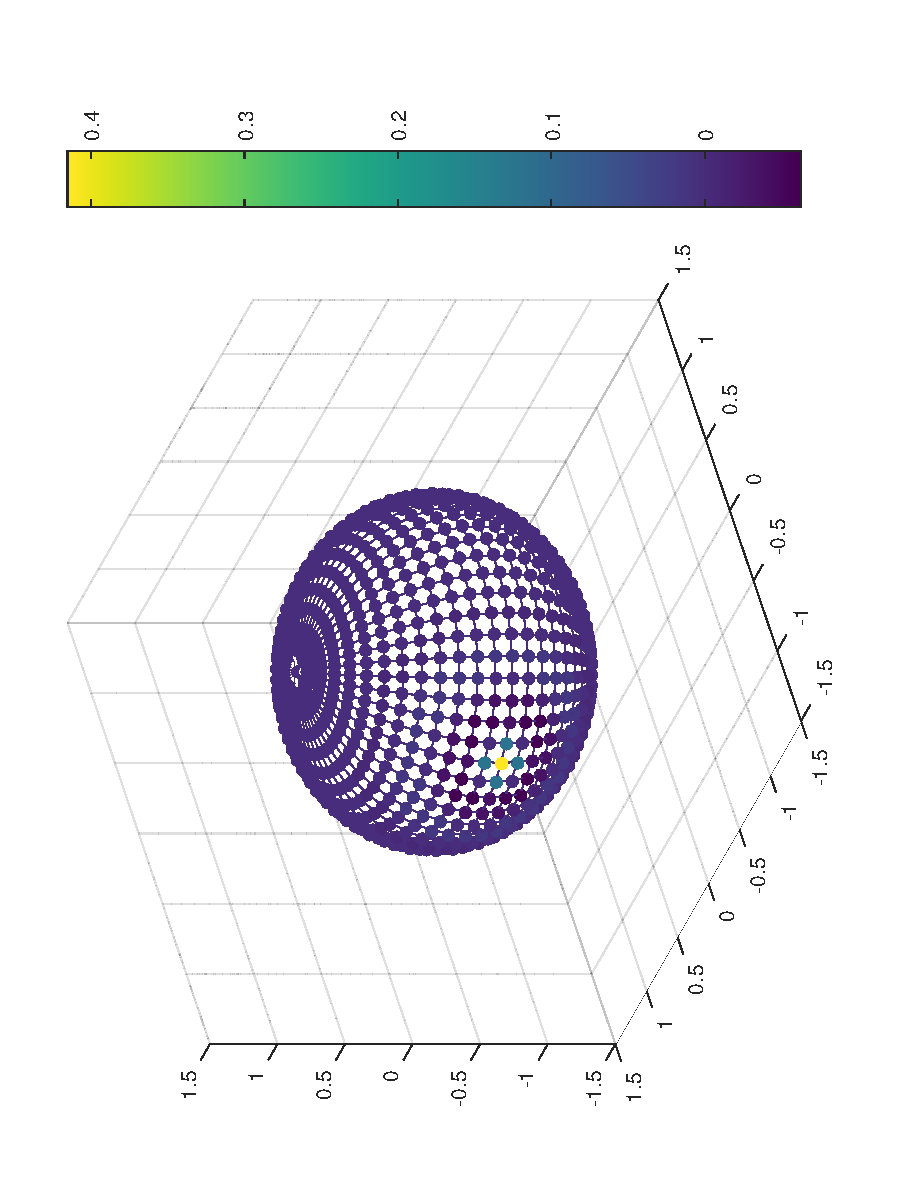
\includegraphics[
        angle=-90,
        origin=c,
        width=\textwidth]{papers/sgwt/images/wavelets/psi_t3_50_25_630.pdf}
        \vspace{-45pt}
        \caption{$\psi_3(v_{630})$-Wavelet eines Kugelgraphen mit 1252 Knoten.}
        \label{fig:sgwt:wavelets:sphere:psi3}
    \end{minipage}
\end{figure}

\begin{figure}
    \begin{minipage}[b]{0.49\textwidth}
        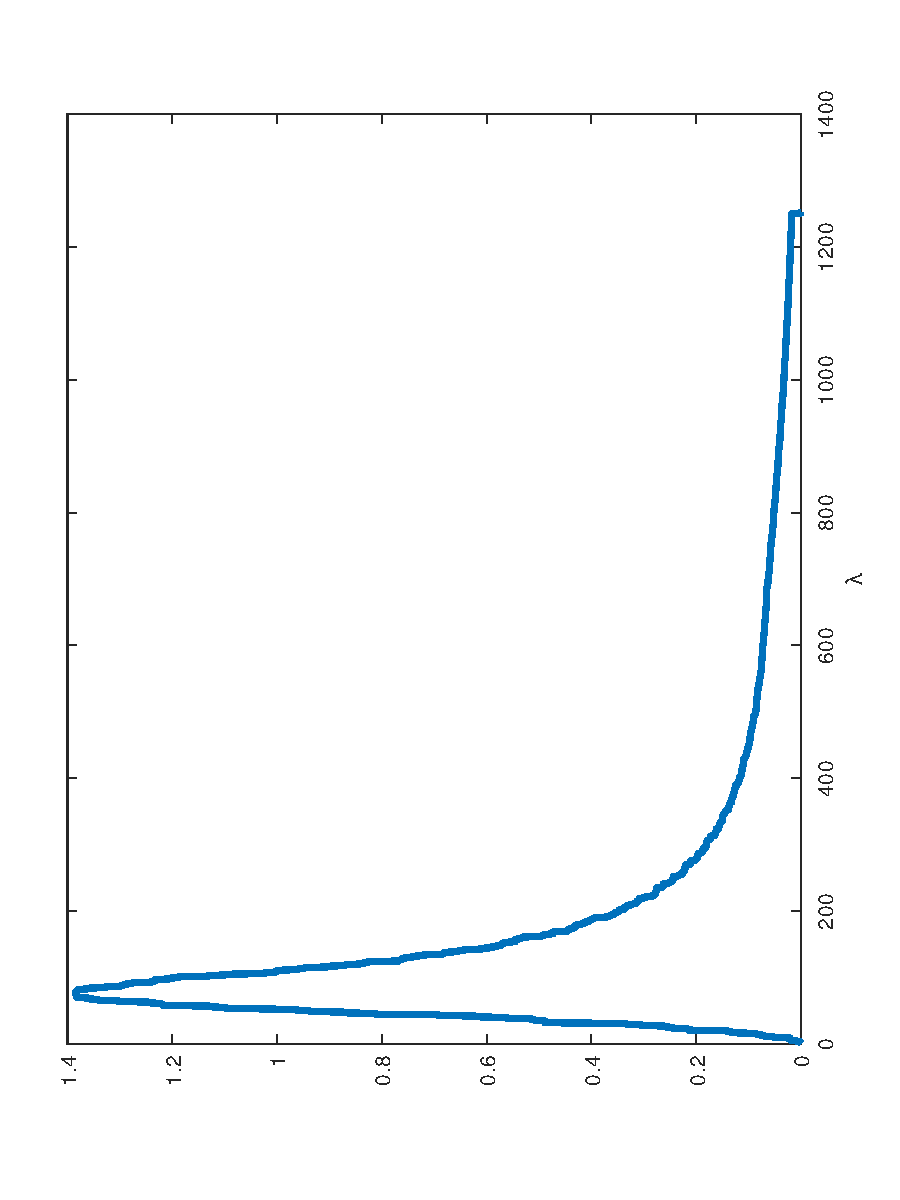
\includegraphics[
        angle=-90,
        origin=c,
        width=\textwidth]{papers/sgwt/images/wavelets/gt4.pdf}
        \vspace{-45pt}
        \caption{Die Kernelfunktion $g(t_4\lambda)$ eines Kugelgraphen mit 1252 
            Knoten und $t_4 = 1.89148$.}
        \label{fig:sgwt:wavelets:sphere:gt4}
    \end{minipage}
    ~
    \begin{minipage}[b]{0.49\textwidth}
        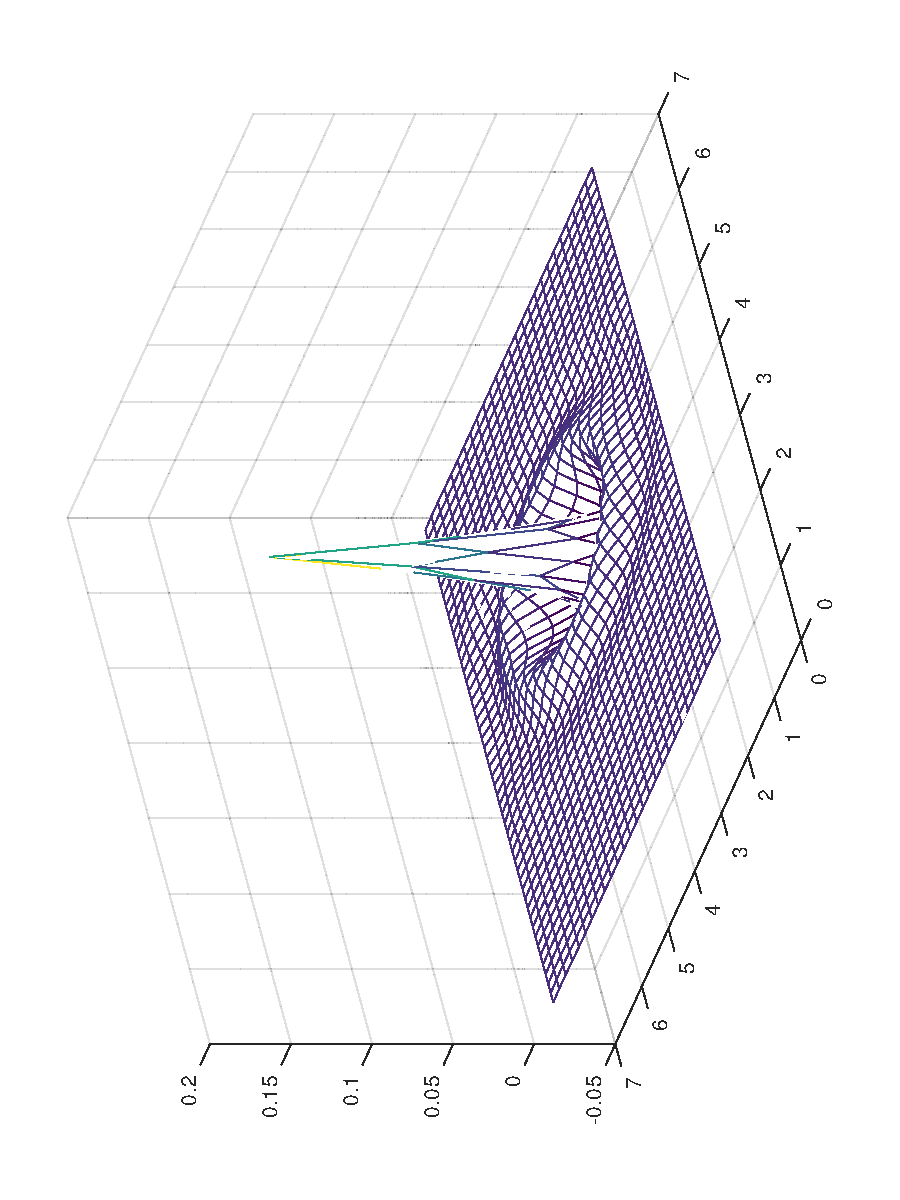
\includegraphics[
        angle=-90,
        origin=c,
        width=\textwidth]{papers/sgwt/images/wavelets/psi_t4_50_25_630_flat.pdf}
        \vspace{-45pt}
        \caption{$\psi_4(v_{630})$-Wavelet eines Kugelgraphen mit 1252 Knoten.}
        \label{fig:sgwt:wavelets:sphere:psi4:flat}
    \end{minipage}
    ~
    \begin{minipage}[b]{\textwidth}
        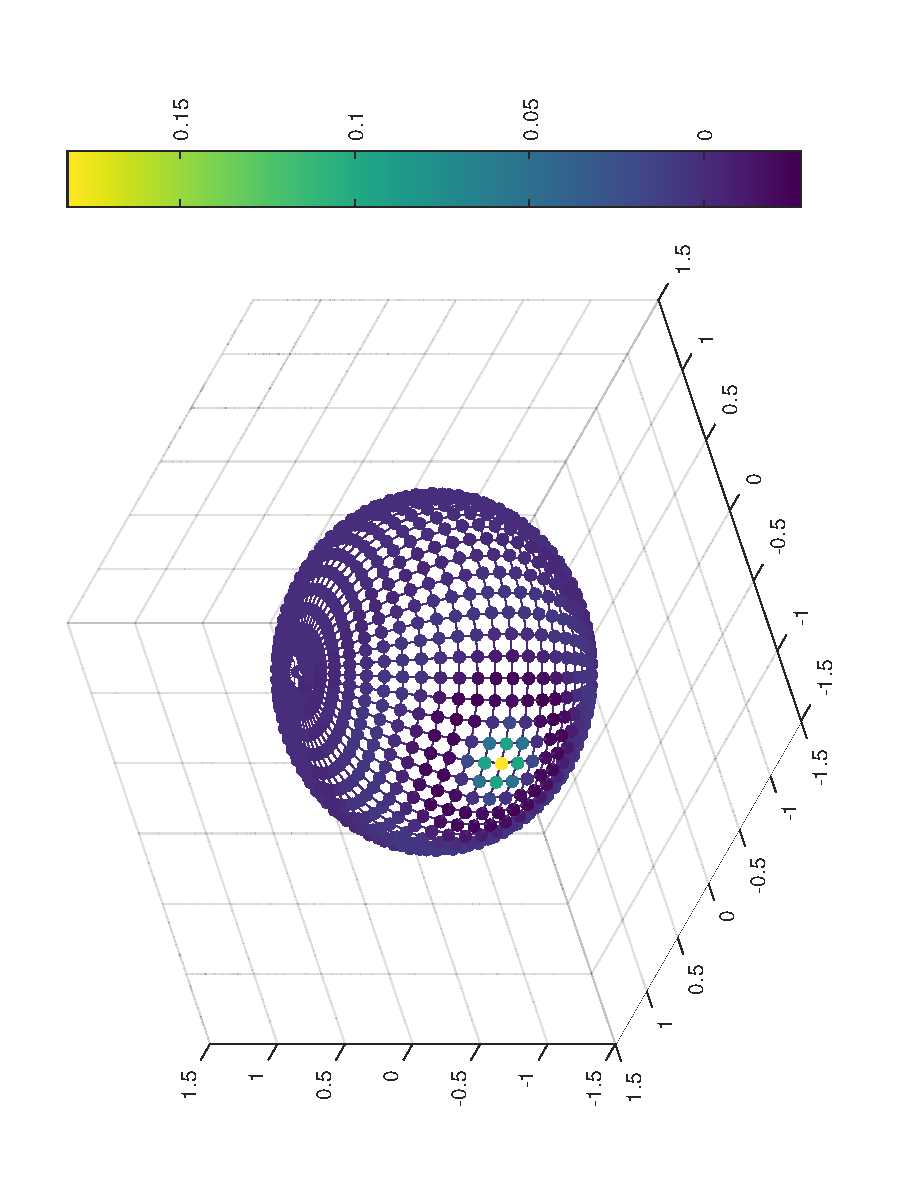
\includegraphics[
        angle=-90,
        origin=c,
        width=\textwidth]{papers/sgwt/images/wavelets/psi_t4_50_25_630.pdf}
        \vspace{-45pt}
        \caption{$\psi_4(v_{630})$-Wavelet eines Kugelgraphen mit 1252 Knoten.}
        \label{fig:sgwt:wavelets:sphere:psi4}
    \end{minipage}
\end{figure}

\begin{figure}
    \begin{minipage}[b]{0.49\textwidth}
        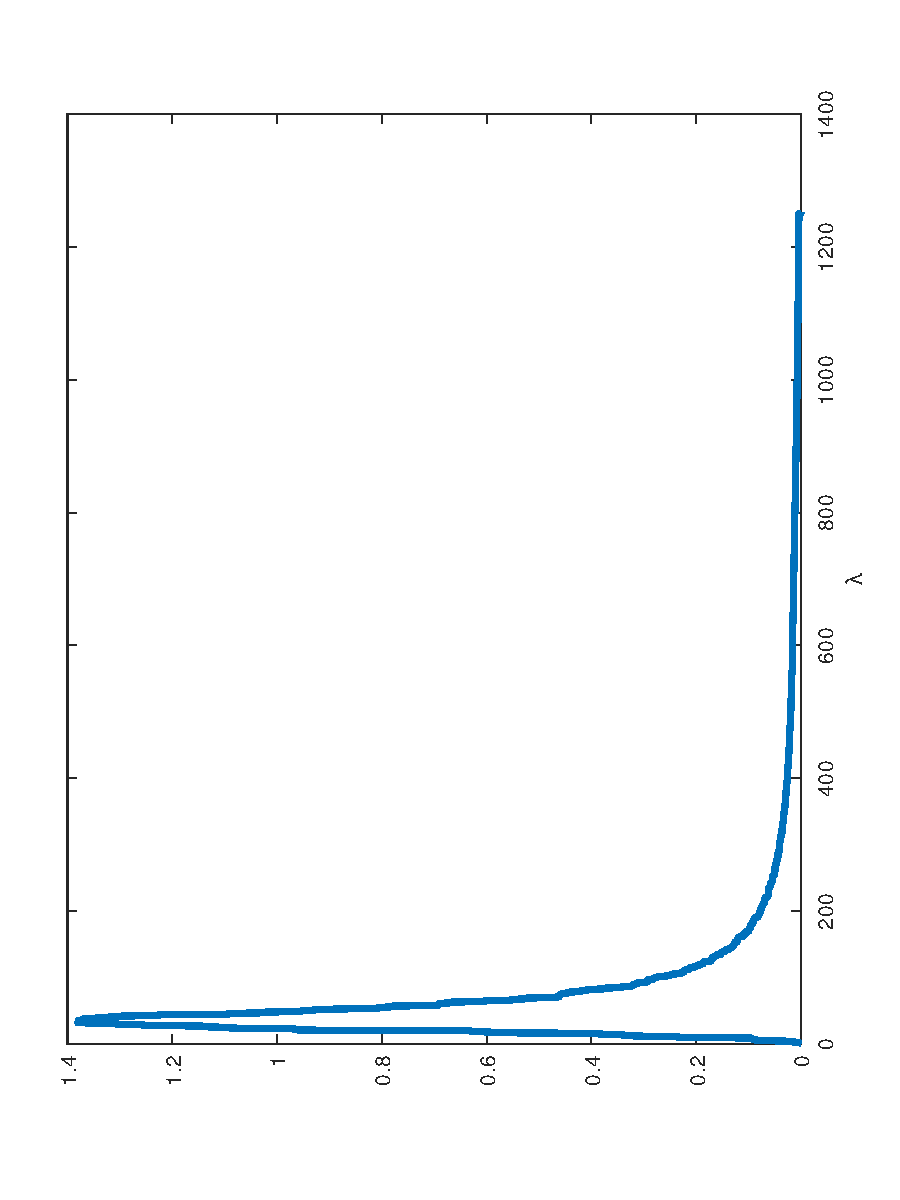
\includegraphics[
        angle=-90,
        origin=c,
        width=\textwidth]{papers/sgwt/images/wavelets/gt5.pdf}
        \vspace{-45pt}
        \caption{Die Kernelfunktion $g(t_5\lambda)$ eines Kugelgraphen mit 1252 
            Knoten und $t_5 = 4$.}
        \label{fig:sgwt:wavelets:sphere:gt5}
    \end{minipage}
    ~
    \begin{minipage}[b]{0.49\textwidth}
        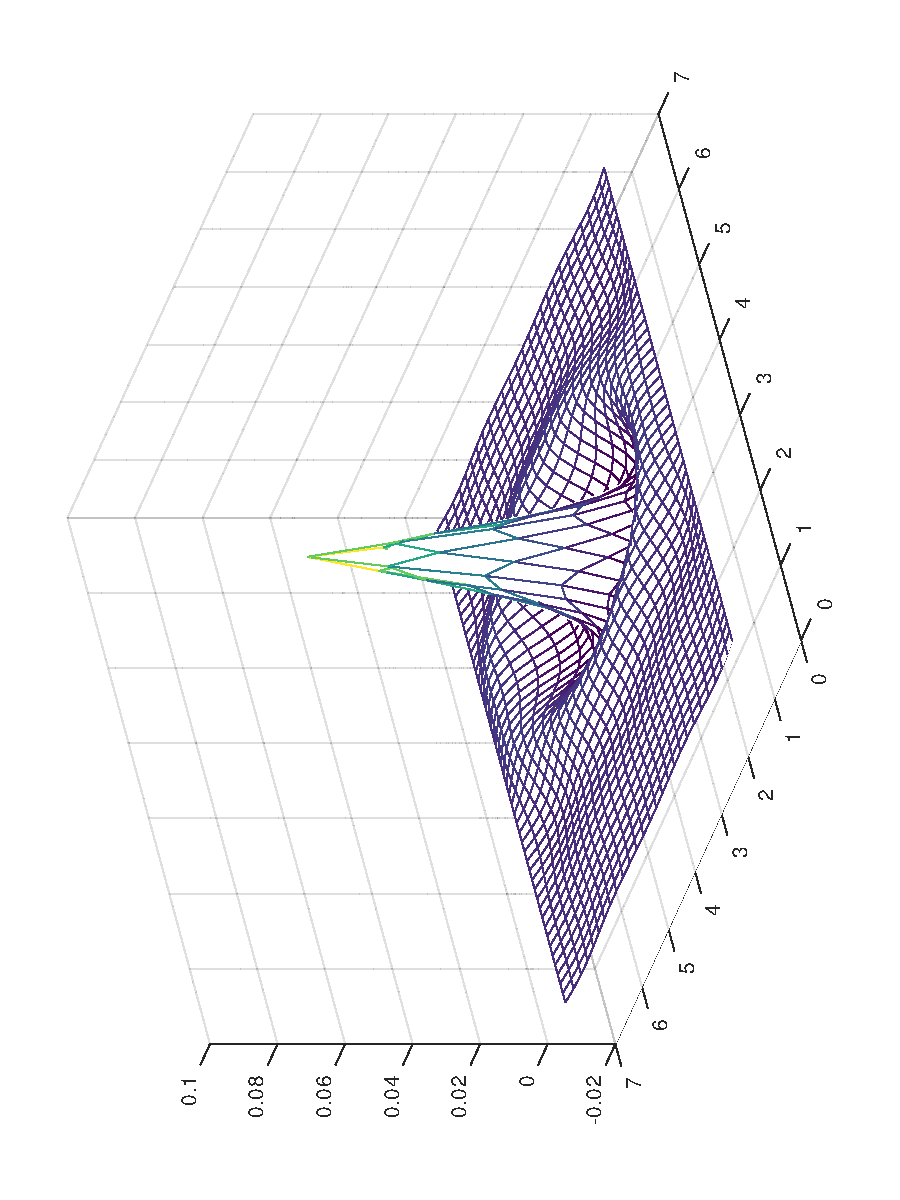
\includegraphics[
        angle=-90,
        origin=c,
        width=\textwidth]{papers/sgwt/images/wavelets/psi_t5_50_25_630_flat.pdf}
        \vspace{-45pt}
        \caption{$\psi_5(v_{630})$-Wavelet eines Kugelgraphen mit 1252 Knoten.}
        \label{fig:sgwt:wavelets:sphere:psi5:flat}
    \end{minipage}
    ~
    \begin{minipage}[b]{\textwidth}
        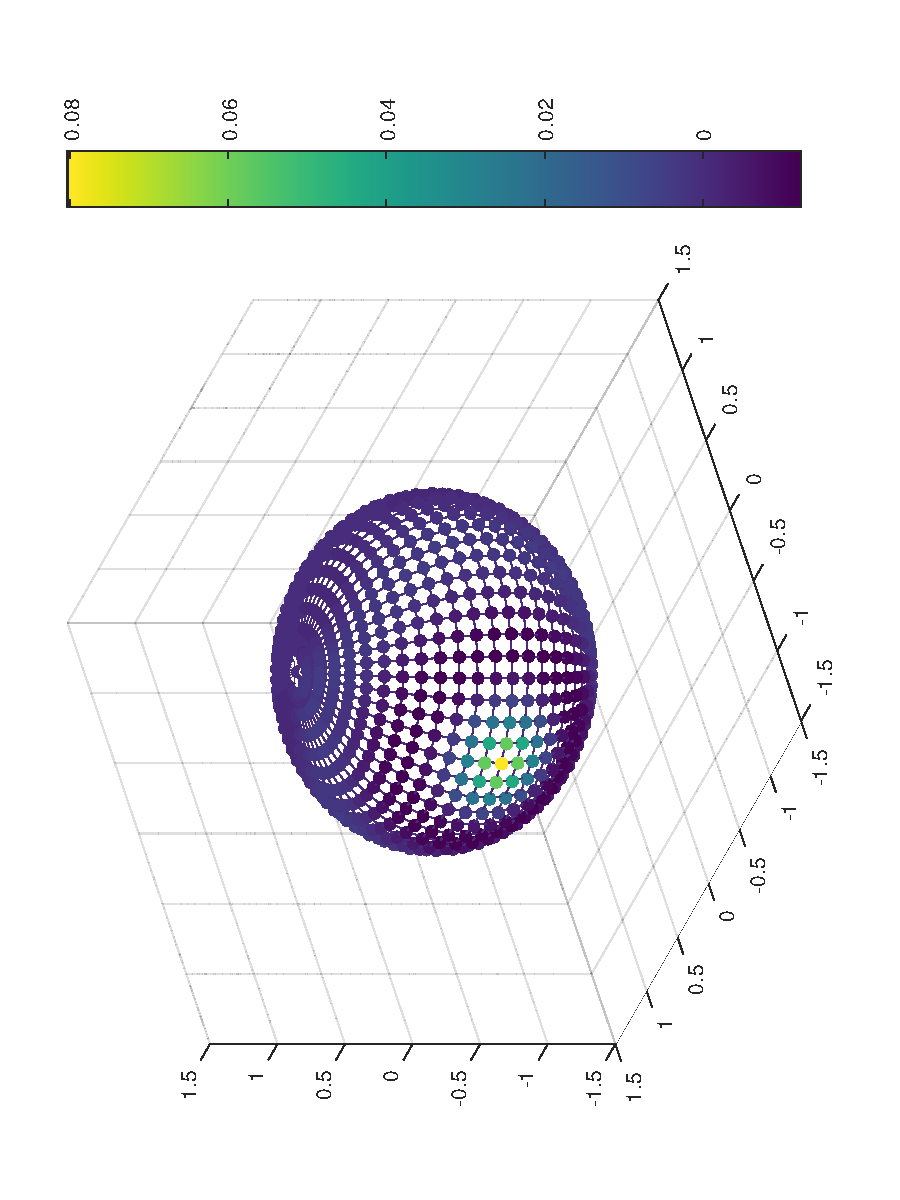
\includegraphics[
        angle=-90,
        origin=c,
        width=\textwidth]{papers/sgwt/images/wavelets/psi_t5_50_25_630.pdf}
        \vspace{-45pt}
        \caption{$\psi_5(v_{630})$-Wavelet eines Kugelgraphen mit 1252 Knoten.}
        \label{fig:sgwt:wavelets:sphere:psi5}
    \end{minipage}
\end{figure}

\begin{figure}
    \begin{minipage}[b]{0.49\textwidth}
        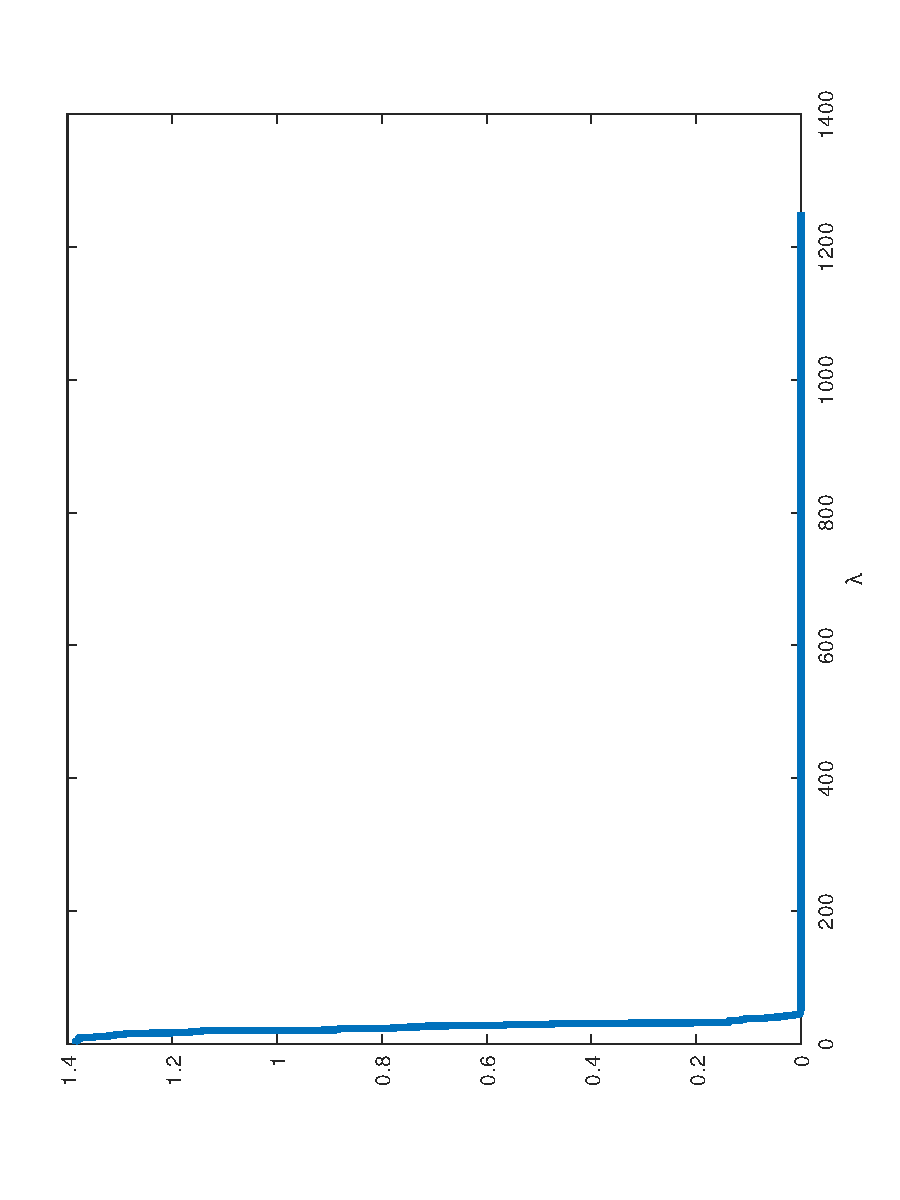
\includegraphics[
        angle=-90,
        origin=c,
        width=\textwidth]{papers/sgwt/images/wavelets/h.pdf}
        \vspace{-45pt}
        \caption{Die Kernelfunktion $h(\lambda)$ eines Kugelgraphen mit 1252 
            Knoten.}
        \label{fig:sgwt:wavelets:sphere:h}
    \end{minipage}
    ~
    \begin{minipage}[b]{0.49\textwidth}
        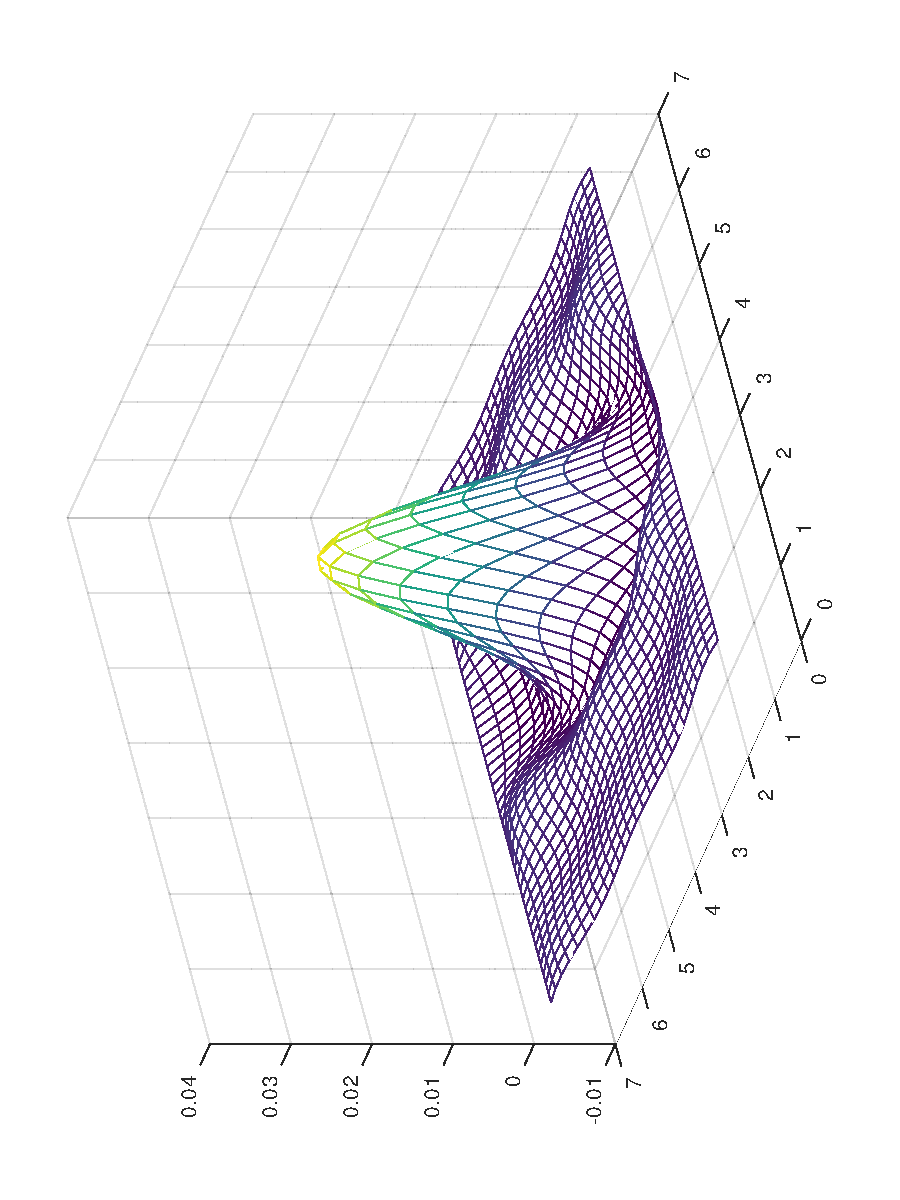
\includegraphics[
        angle=-90,
        origin=c,
        width=\textwidth]{papers/sgwt/images/wavelets/phi_50_25_630_flat.pdf}
        \vspace{-45pt}
        \caption{$\phi(v_{630})$-Wavelet eines Kugelgraphen mit 1252 Knoten.}
        \label{fig:sgwt:wavelets:sphere:phi:flat}
    \end{minipage}
    ~
    \begin{minipage}[b]{\textwidth}
        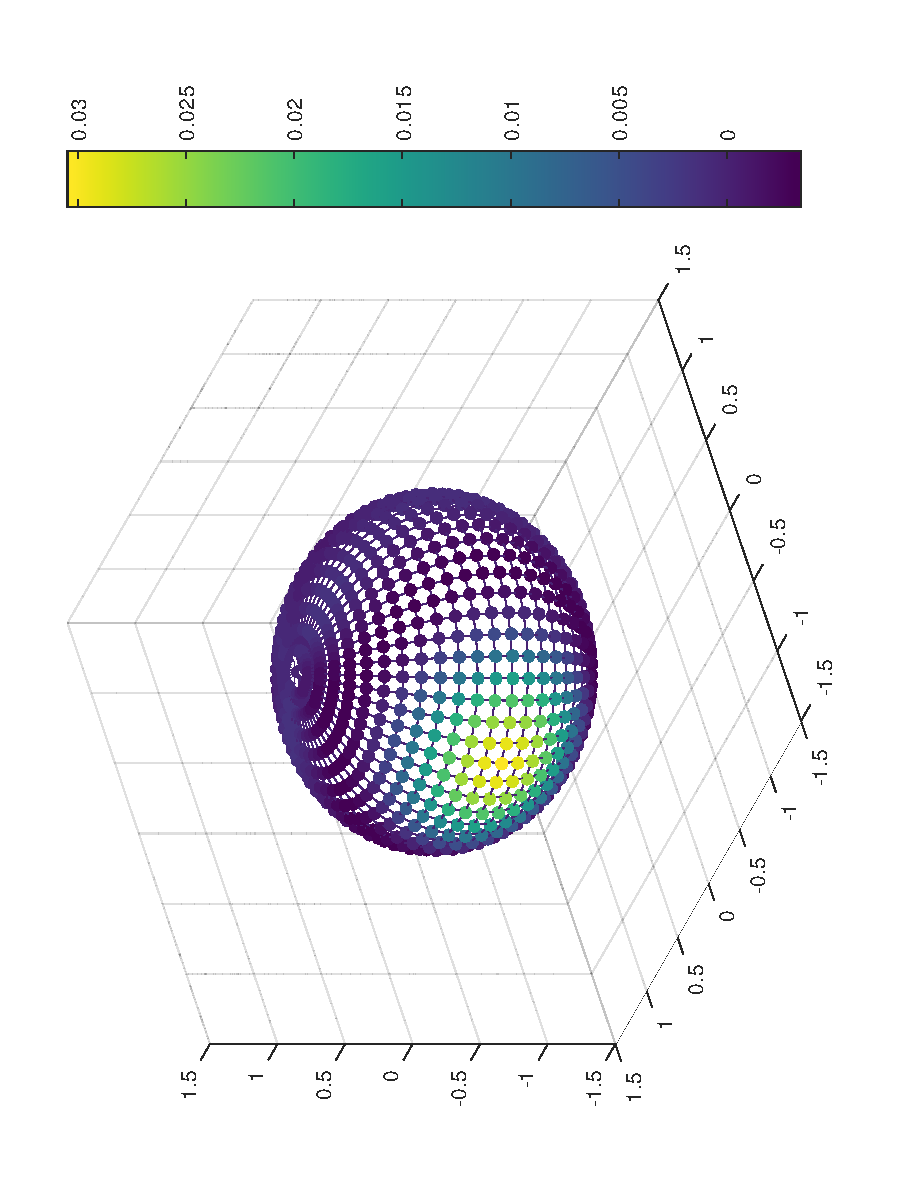
\includegraphics[
        angle=-90,
        origin=c,
        width=\textwidth]{papers/sgwt/images/wavelets/phi_50_25_630.pdf}
        \vspace{-45pt}
        \caption{$\phi(v_{630})$-Wavelet eines Kugelgraphen mit 1252 Knoten.}
        \label{fig:sgwt:wavelets:sphere:phi}
    \end{minipage}
\end{figure}

\subsubsection{Kernelfunktionen}

Um dieses Problem zu l\"osen nehmen wir eine Kernelfunktion $g(\lambda)$, 
welche die Eigenschaften $g(0) = 0$ und $\lim_{\lambda\to\infty} g(x) = 0$ 
erf\"ullt. Mit Hilfe dieses Bandpasses k\"onnen wir die Eigenwerte bewusst 
delokalisieren. Wenn wir nun zus\"atzlich die Eigenwerte mit einem 
Skalierungsfaktor $t$ multiplizieren, erhalten wir auch eine 
M\"oglichkeit, das Spektrum zu verschieben. Obwohl $t$ ein kontinuierlicher 
Faktor ist, werden wir uns in der Praxis auf $J$ Faktoren, also eine endliche 
Anzahl $\{t_j\}^J_{j=1}$, beschr\"anken m\"ussen.

Wir haben jetzt nur noch das Problem, dass $\lambda_0 = 0$ gilt. Wir verlieren 
also den konstanten Anteil der zu analysierenden und synthetisierenden 
Funktion. Um das zu umgehen nehmen brauchen wir eine zus\"atzliche 
Kernelfunktion $h(\lambda)$ mit den Eigenschaften $h(0) > 0$ und 
$\lim_{\lambda\to\infty} = 0$.

Die in~\cref{sec:sgwt:spectralanalysis} vorgestellten Eigenfunktionen 
k\"onnen wir direkt nutzen um eine Graph Fourier Transformation zu definieren. 
Wir ersetzen bei der Fourier Transformation einfach die Exponentialfunktion 
oder Kugelfunktionen durch die Eigenvektoren der Laplace Matrix
\begin{equation*}
\hat{f} = \langle \chi, f \rangle = \sum_{n = 1}^{N} \chi^*(n)f(n).
\end{equation*}
Wenn wir, wie zum Beispiel in \texttt{octave} \"ublich, die Eigenvektoren als 
Spalten einer Matrix
\begin{equation}
\chi = 
\left[
\begin{pmatrix}\\\chi_0\\\\\end{pmatrix}
\begin{pmatrix}\\\chi_1\\\\\end{pmatrix}
\begin{pmatrix}\\\chi_2\\\\\end{pmatrix}
\cdots
\begin{pmatrix}\\\chi_{N-1}\\\\\end{pmatrix}
\right]
\end{equation}
zur Verf\"ugung haben, k\"onnen wir die Transformation 
einfach durch eine Matrix-Vektor Multiplikation ersetzen
\begin{equation*}
\hat{f} = \chi^* f.
\end{equation*}
Die R\"ucktransformation ist dann auch wieder analog der Fouriertheorie
\begin{equation*}
f = \chi \hat{f}.
\end{equation*}

\subsection{Graph Wavelets: Lokalisierung\label{subsec:sgwt:gwt:localizing}}

Mit der Graph Fourier Transformation k\"onnen wir nun Funktionen auf Graphen 
analysieren und dann auch wieder synthetisieren. Mit Hilfe von Wavelets haben 
wir aber bereits gesehen, dass damit auch eine Lokalisierung m\"oglich ist. 
Graphen haben da den Nachteil, dass die Knoten keine inh\"arente Reihenfolge 
haben. Es ist also nicht klar was mit $f(x - h)$ gemeint ist. Wir haben 
allerdings in~\cref{eq:sgwt:lambda:series} eine Reihenfolge f\"ur die 
Eigenwerte der Laplace Matrix eines Graphen definiert. Die Eigenwerte sind 
allerdings komplett lokalisiert, sie kommen also einem Dirac-Stoss an 
einem Knoten gleich.

\subsection{Graph Wavelets: Skalierung\label{subsec:sgwt:gwt:scaling}}

\subsection{Frames}

Mit $h(\lambda)$ und den $J$ skalierten $g(t\lambda)$ haben wir also $J + 1$ 
Kernelfunktionen f\"ur die Analyse und Synthese zur Verf\"ugung. Wir arbeiten 
also mit einem Frame. Die Grenzen sind dabei gegeben als
\begin{align*}
A &= \min_{\lambda \in \left[0, \lambda_{N-1}\right]} f(\lambda) \\
B &= \max_{\lambda \in \left[0, \lambda_{N-1}\right]} f(\lambda) \\
\text{mit } f(\lambda) &= h(\lambda)^2 + \sum_{j = 1}^{J} g(t_j\lambda)^2.
\end{align*}

\subsection{\texorpdfstring{$\psi_j$}{psi} und \texorpdfstring{$\phi$}{phi}}
Damit lassen sich nun unsere Wavelets $\psi_j$ und $\phi$ wie folgt konstruieren
\begin{align}
\psi_j = \chi \diag{g(t_j\lambda)} \chi' 
\label{eq:sgwt:psi}
\\
\phi = \chi \diag{h(\lambda)} \chi'.
\label{eq:sgwt:phi}
\end{align}
Zur Veranschaulichung sehen wir hier die Wavelets eines Kreisgraphen 
in~\cref{fig:sgwt:wavelets:ring0,fig:sgwt:wavelets:ring1,fig:sgwt:wavelets:ring2,fig:sgwt:wavelets:ring3,fig:sgwt:wavelets:ring4,fig:sgwt:wavelets:ring5},
 eines Streckengraphen 
in~\cref{fig:sgwt:wavelets:line0,fig:sgwt:wavelets:line1,fig:sgwt:wavelets:line2,fig:sgwt:wavelets:line3,fig:sgwt:wavelets:line4,fig:sgwt:wavelets:line5}
 und eines Kugelgraphen 
in~\cref{fig:sgwt:wavelets:sphere0,fig:sgwt:wavelets:sphere1,fig:sgwt:wavelets:sphere2,fig:sgwt:wavelets:sphere3,fig:sgwt:wavelets:sphere4,fig:sgwt:wavelets:sphere5}.
Gut zu erkennen ist dabei, dass der Kreisgraph die wohl beste Approximation der 
bisherigen Wavelettheorie ist. Beim Streckengraph fehlt die Periodisierung, die 
wir durch die Verbindungskante des Start- und Endknoten beim Kreisgraphen 
erreicht haben. Auch beim Kugelgraphen wird klar, dass die Pole, aufgrund ihres 
viel gr\"osseren Grades, deutlich st\"arker gewichtet werden und es daher zu 
einer Verzerrung der Wavelets in Richtung der Pole kommt.

\begin{figure}
    \centering
    \begin{minipage}[b]{0.49\textwidth}
        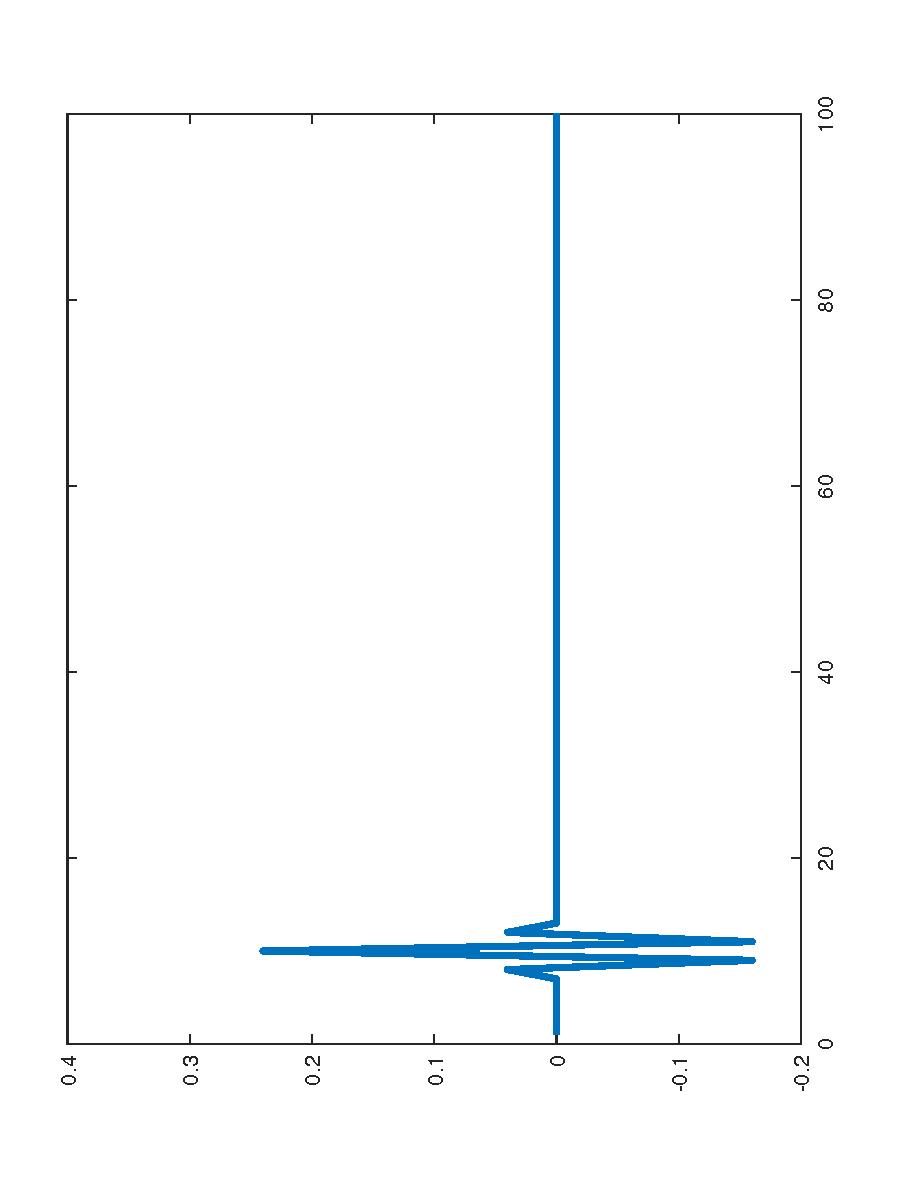
\includegraphics[
        angle=-90,
        origin=c,
        width=\textwidth]{papers/sgwt/images/wavelets-psi-1-10.pdf}
        \vspace{-45pt}
        \caption{$\psi_1(v_{10})$-Wavelets eines Kreisgraphen mit 100 Knoten.}
        \label{fig:sgwt:wavelets:ring0}
    \end{minipage}
    ~
    \begin{minipage}[b]{0.49\textwidth}
        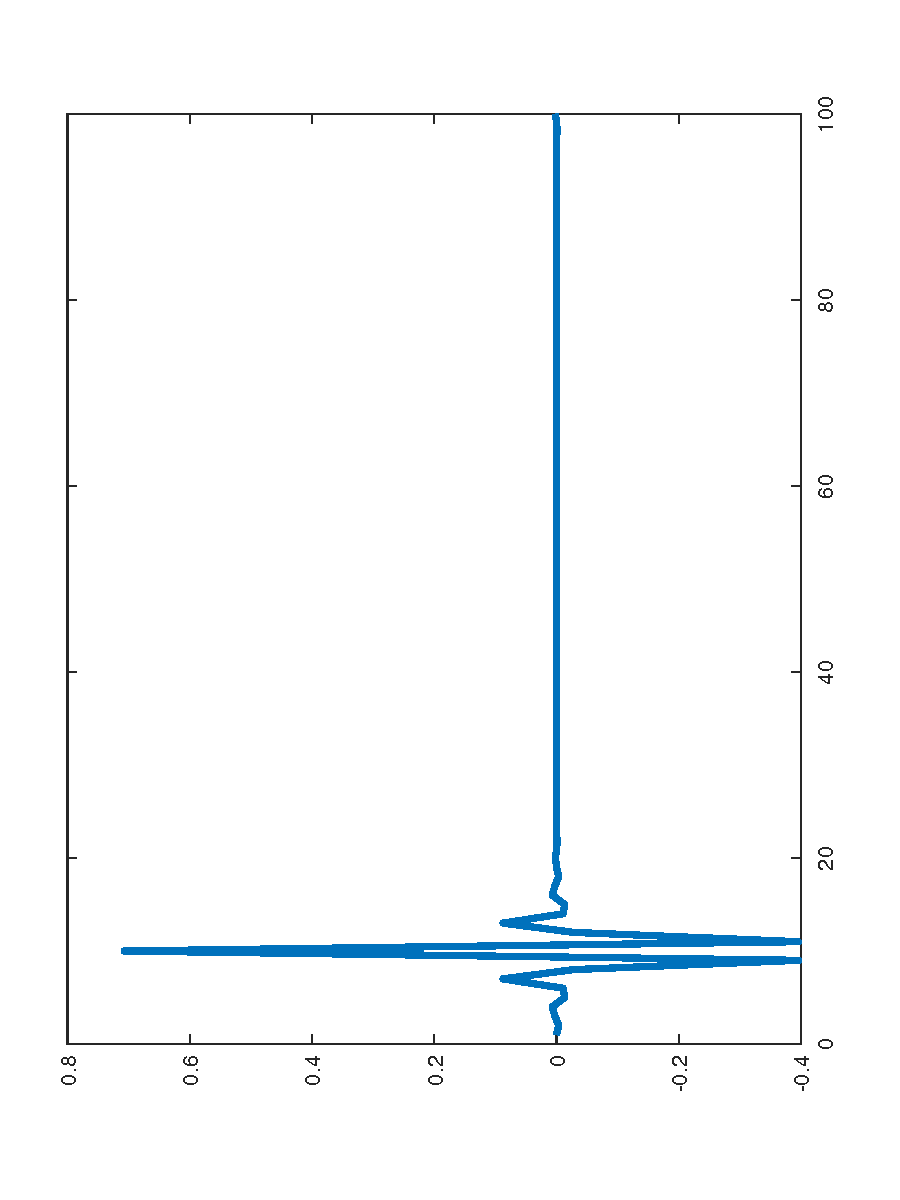
\includegraphics[
        angle=-90,
        origin=c,
        width=\textwidth]{papers/sgwt/images/wavelets-psi-2-10.pdf}
        \vspace{-45pt}
        \caption{$\psi_2(v_{10})$-Wavelets eines Kreisgraphen mit 100 Knoten.}
        \label{fig:sgwt:wavelets:ring1}
    \end{minipage}
    ~
    \begin{minipage}[b]{0.49\textwidth}
        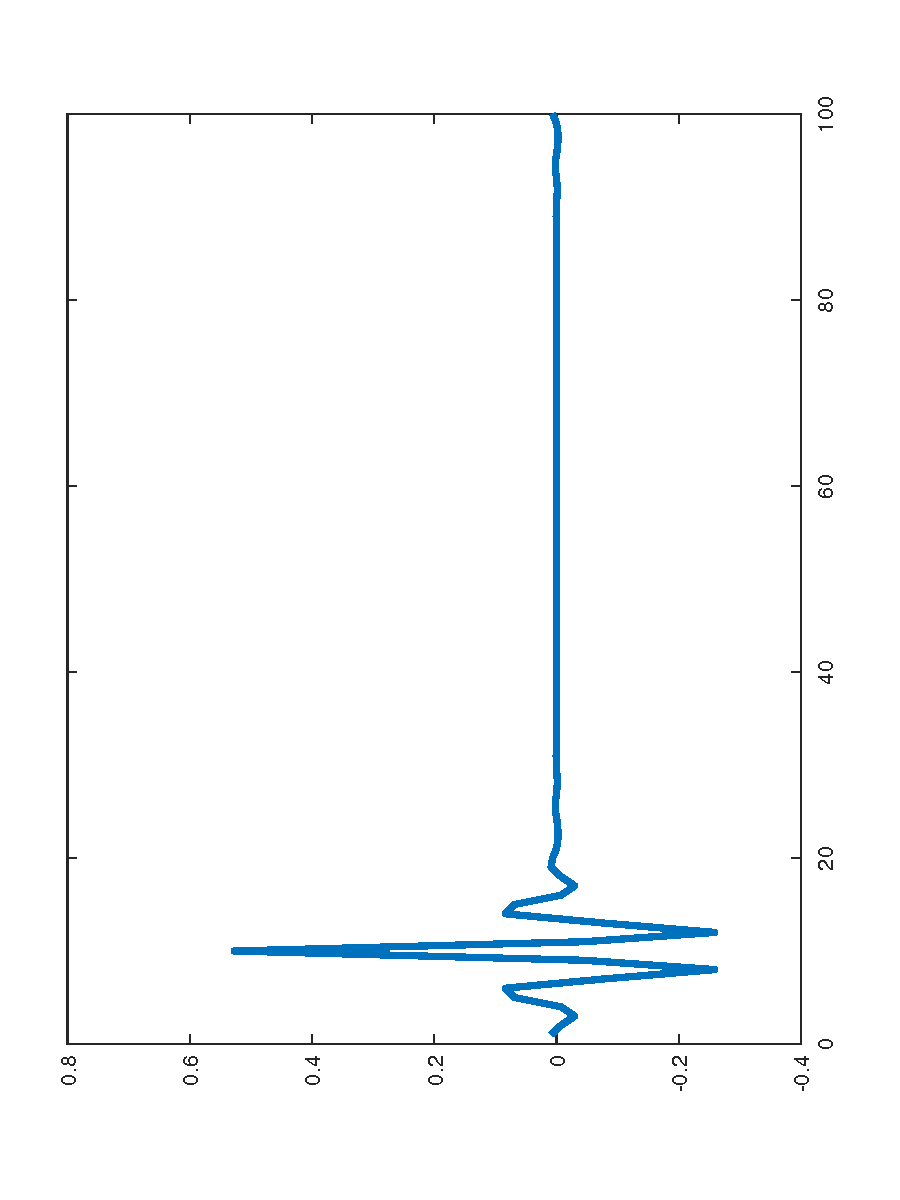
\includegraphics[
        angle=-90,
        origin=c,
        width=\textwidth]{papers/sgwt/images/wavelets-psi-3-10.pdf}
        \vspace{-45pt}
        \caption{$\psi_3(v_{10})$-Wavelets eines Kreisgraphen mit 100 Knoten.}
        \label{fig:sgwt:wavelets:ring2}
    \end{minipage}
    ~
    \begin{minipage}[b]{0.49\textwidth}
        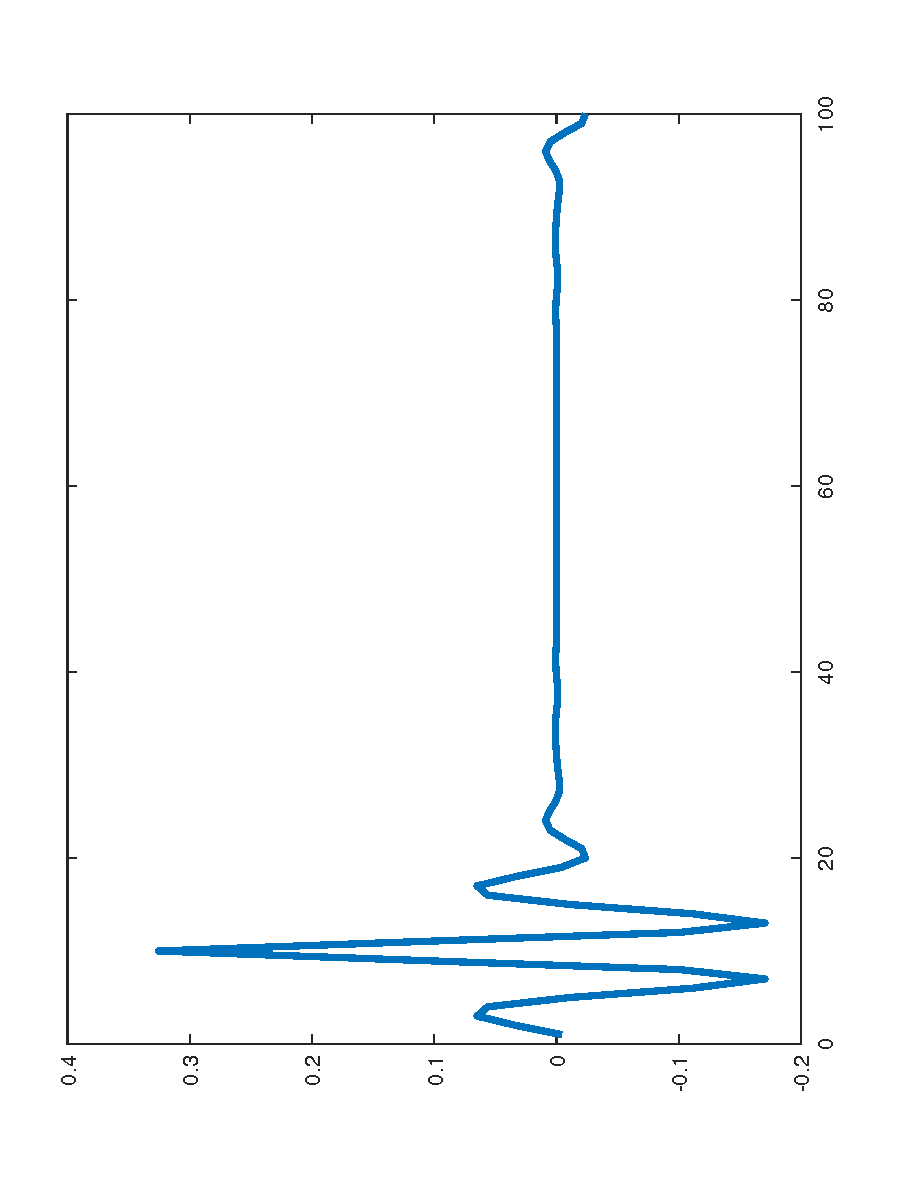
\includegraphics[
        angle=-90,
        origin=c,
        width=\textwidth]{papers/sgwt/images/wavelets-psi-4-10.pdf}
        \vspace{-45pt}
        \caption{$\psi_4(v_{10})$-Wavelets eines Kreisgraphen mit 100 Knoten.}
        \label{fig:sgwt:wavelets:ring3}
    \end{minipage}
    ~
    \begin{minipage}[b]{0.49\textwidth}
        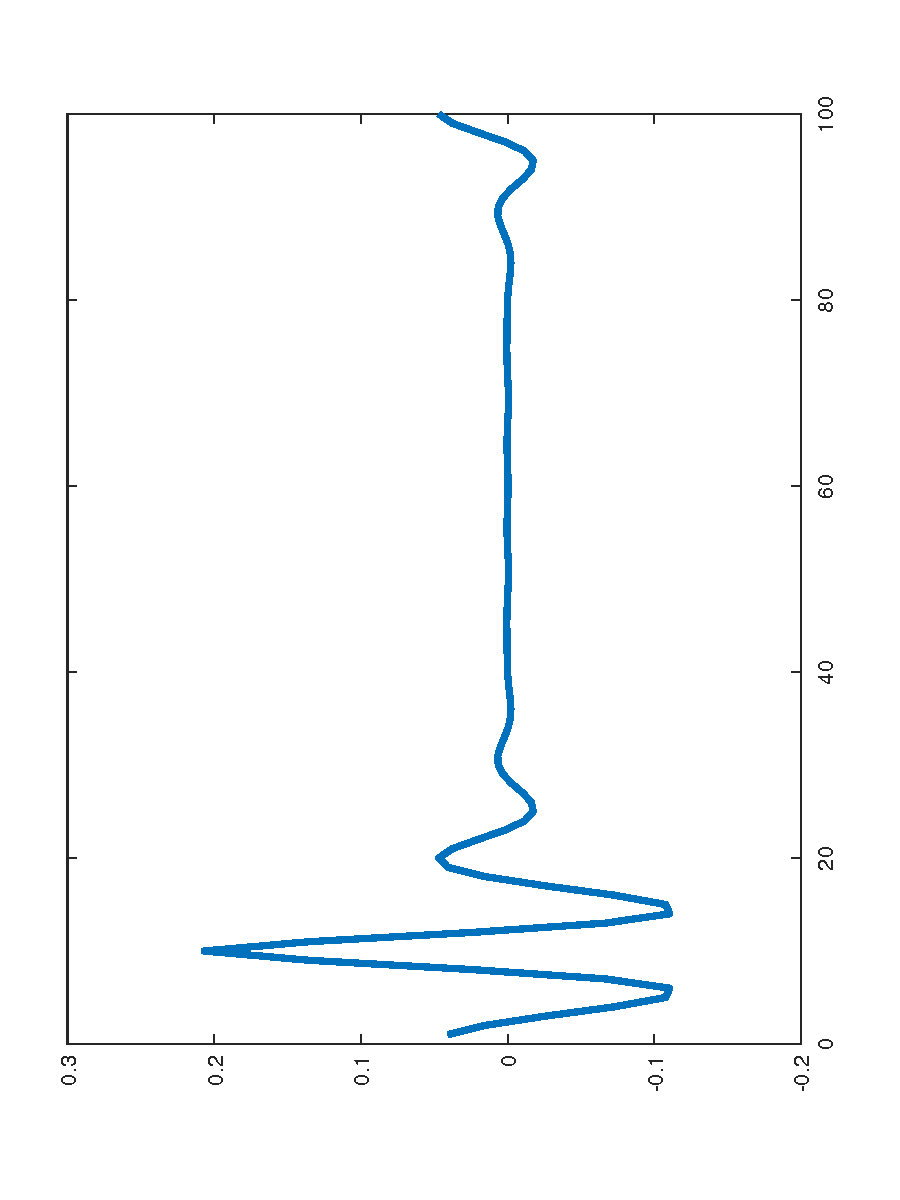
\includegraphics[
        angle=-90,
        origin=c,
        width=\textwidth]{papers/sgwt/images/wavelets-psi-5-10.pdf}
        \vspace{-45pt}
        \caption{$\psi_5(v_{10})$-Wavelets eines Kreisgraphen mit 100 Knoten.}
        \label{fig:sgwt:wavelets:ring4}
    \end{minipage}
    ~
    \begin{minipage}[b]{0.49\textwidth}
        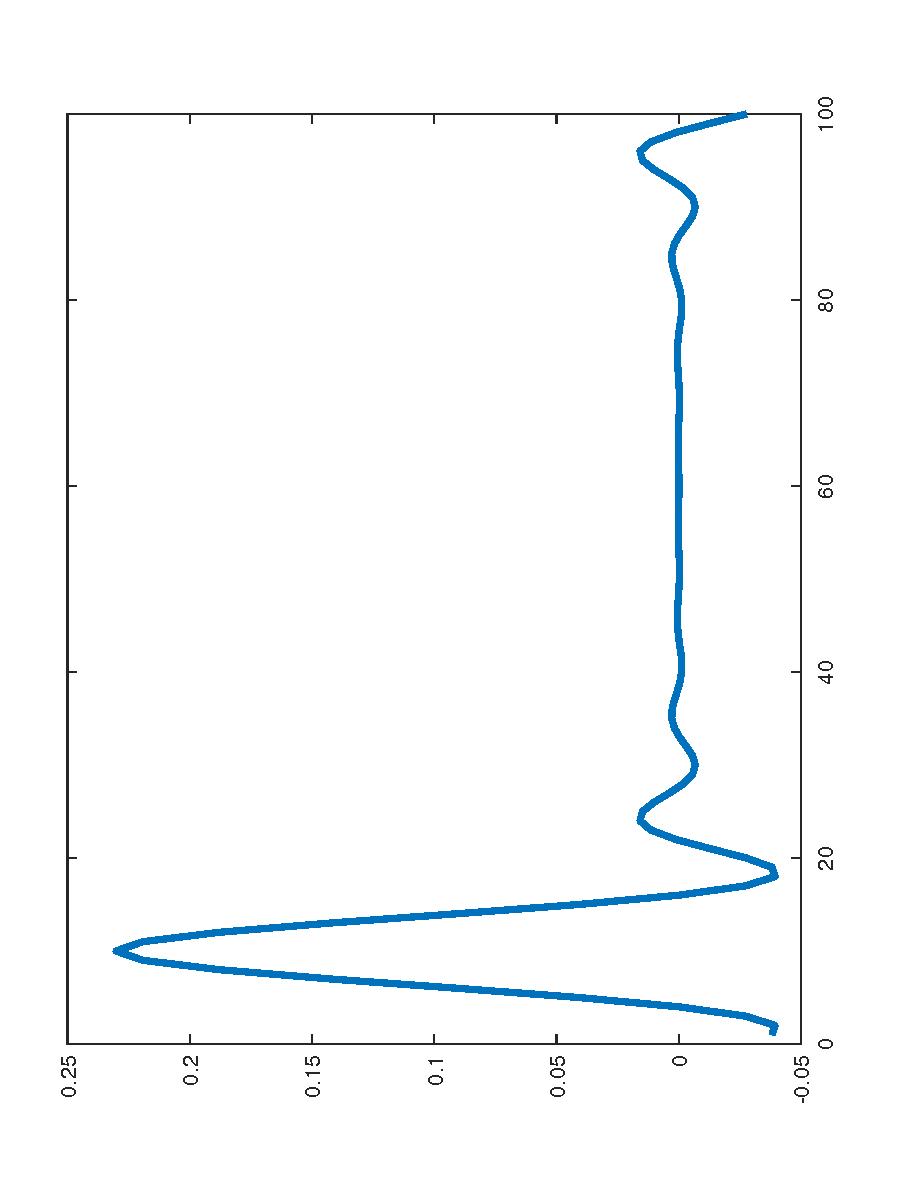
\includegraphics[
        angle=-90,
        origin=c,
        width=\textwidth]{papers/sgwt/images/wavelets-phi-10.pdf}
        \vspace{-45pt}
        \caption{$\phi(v_{10})$-Wavelets eines Kreisgraphen mit 100 Knoten.}
        \label{fig:sgwt:wavelets:ring5}
    \end{minipage}
\end{figure}

\begin{figure}
    \centering
    \begin{minipage}[b]{0.49\textwidth}
        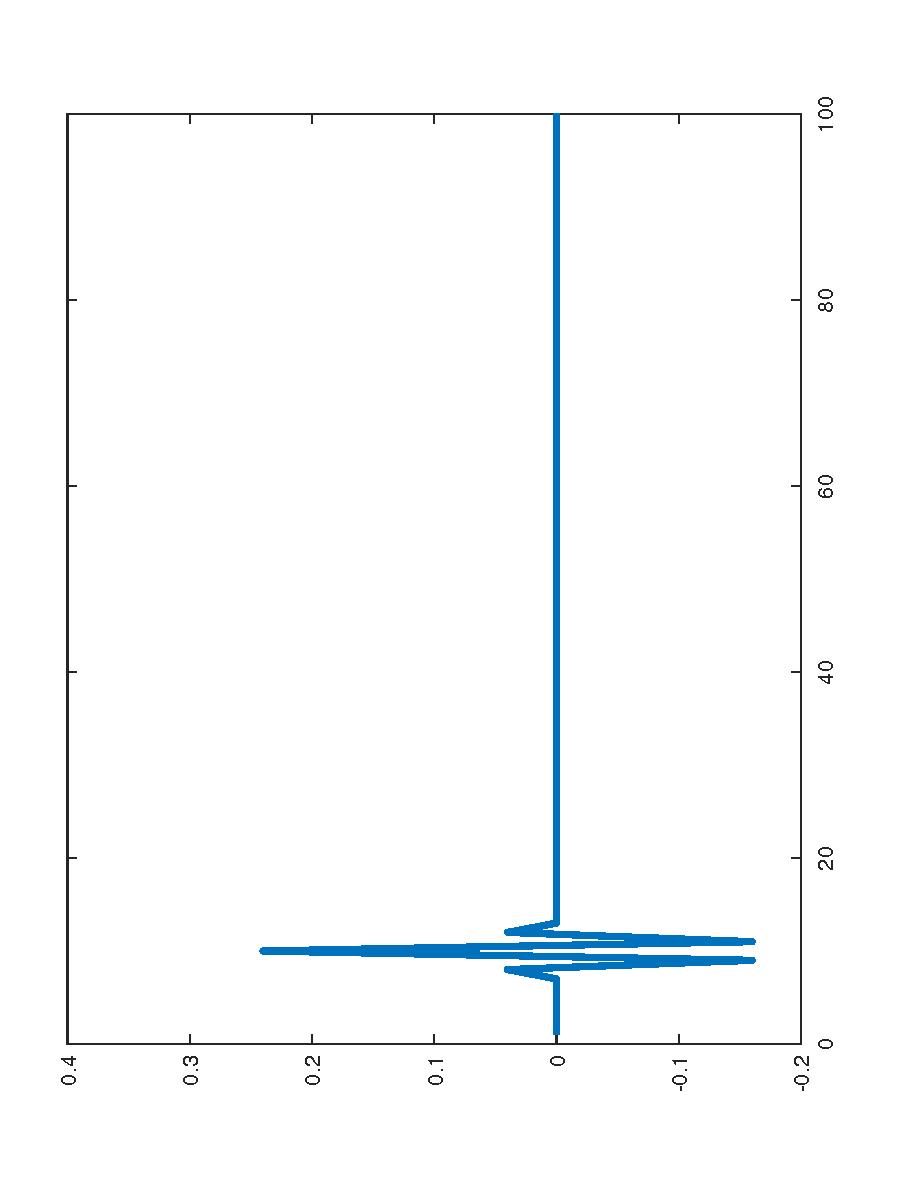
\includegraphics[
        angle=-90,
        origin=c,
        width=\textwidth]{papers/sgwt/images/wavelets-psi-line-1-10.pdf}
        \vspace{-45pt}
        \caption{$\psi_1(v_{10})$-Wavelets eines Streckengraphen mit 100 
        Knoten.}
        \label{fig:sgwt:wavelets:line0}
    \end{minipage}
    ~
    \begin{minipage}[b]{0.49\textwidth}
        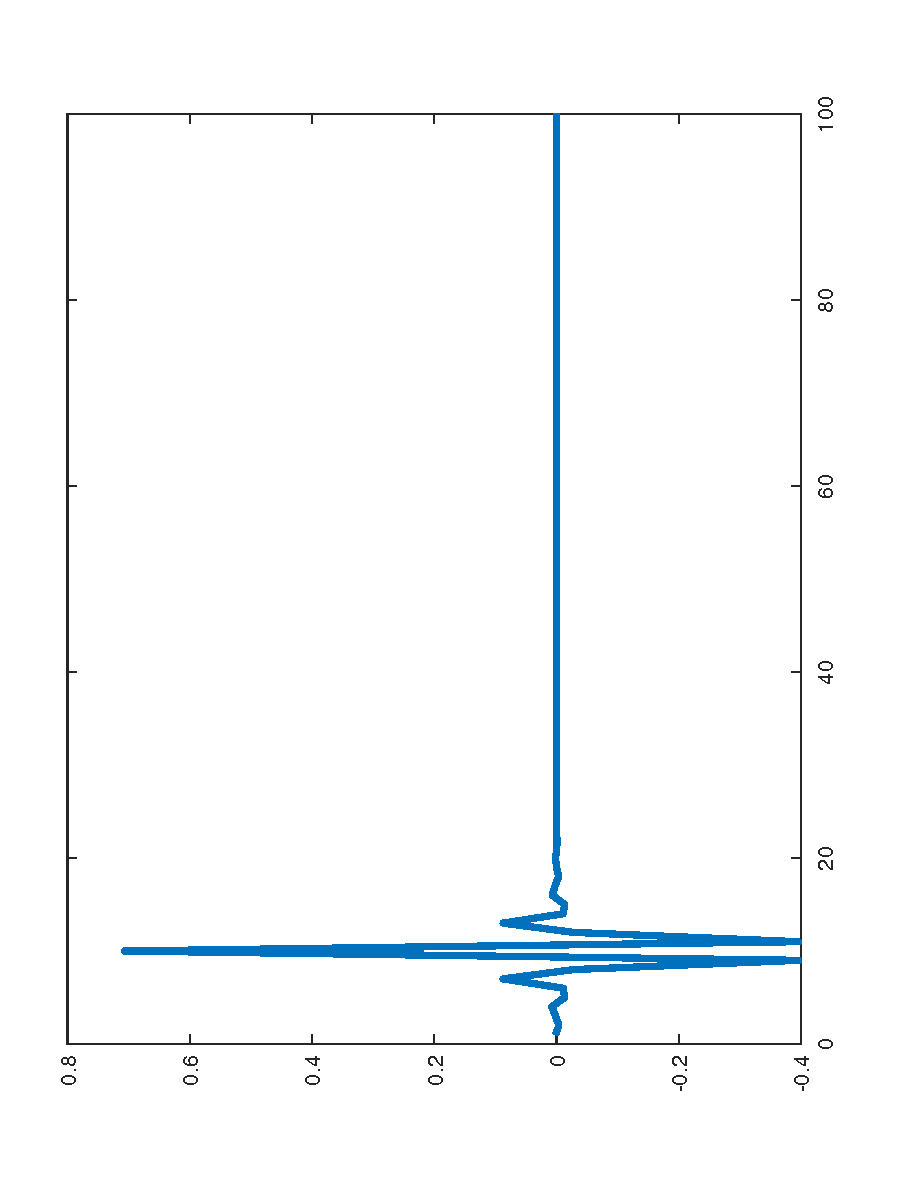
\includegraphics[
        angle=-90,
        origin=c,
        width=\textwidth]{papers/sgwt/images/wavelets-psi-line-2-10.pdf}
        \vspace{-45pt}
        \caption{$\psi_2(v_{10})$-Wavelets eines Streckengraphen mit 100 
        Knoten.}
        \label{fig:sgwt:wavelets:line1}
    \end{minipage}
    ~
    \begin{minipage}[b]{0.49\textwidth}
        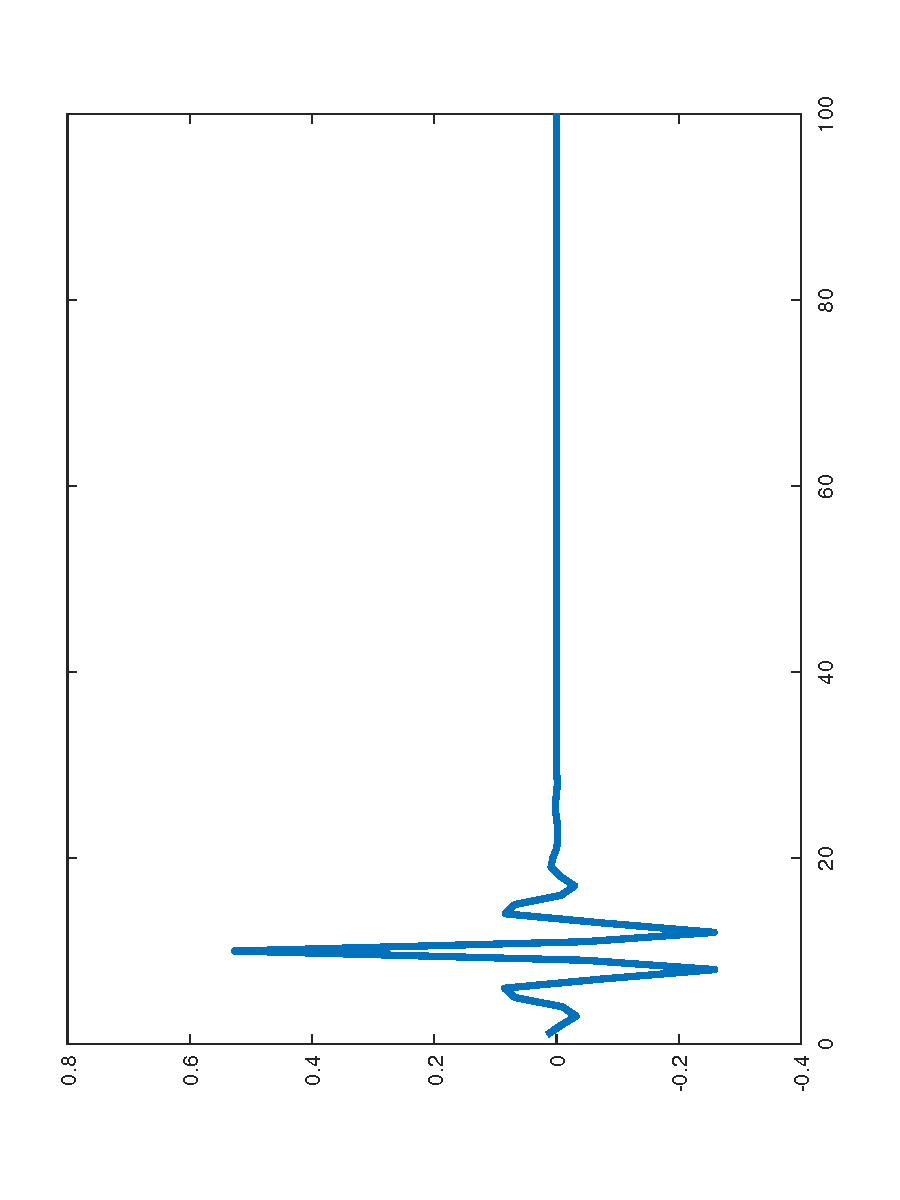
\includegraphics[
        angle=-90,
        origin=c,
        width=\textwidth]{papers/sgwt/images/wavelets-psi-line-3-10.pdf}
        \vspace{-45pt}
        \caption{$\psi_3(v_{10})$-Wavelets eines Streckengraphen mit 100 
        Knoten.}
        \label{fig:sgwt:wavelets:line2}
    \end{minipage}
    ~
    \begin{minipage}[b]{0.49\textwidth}
        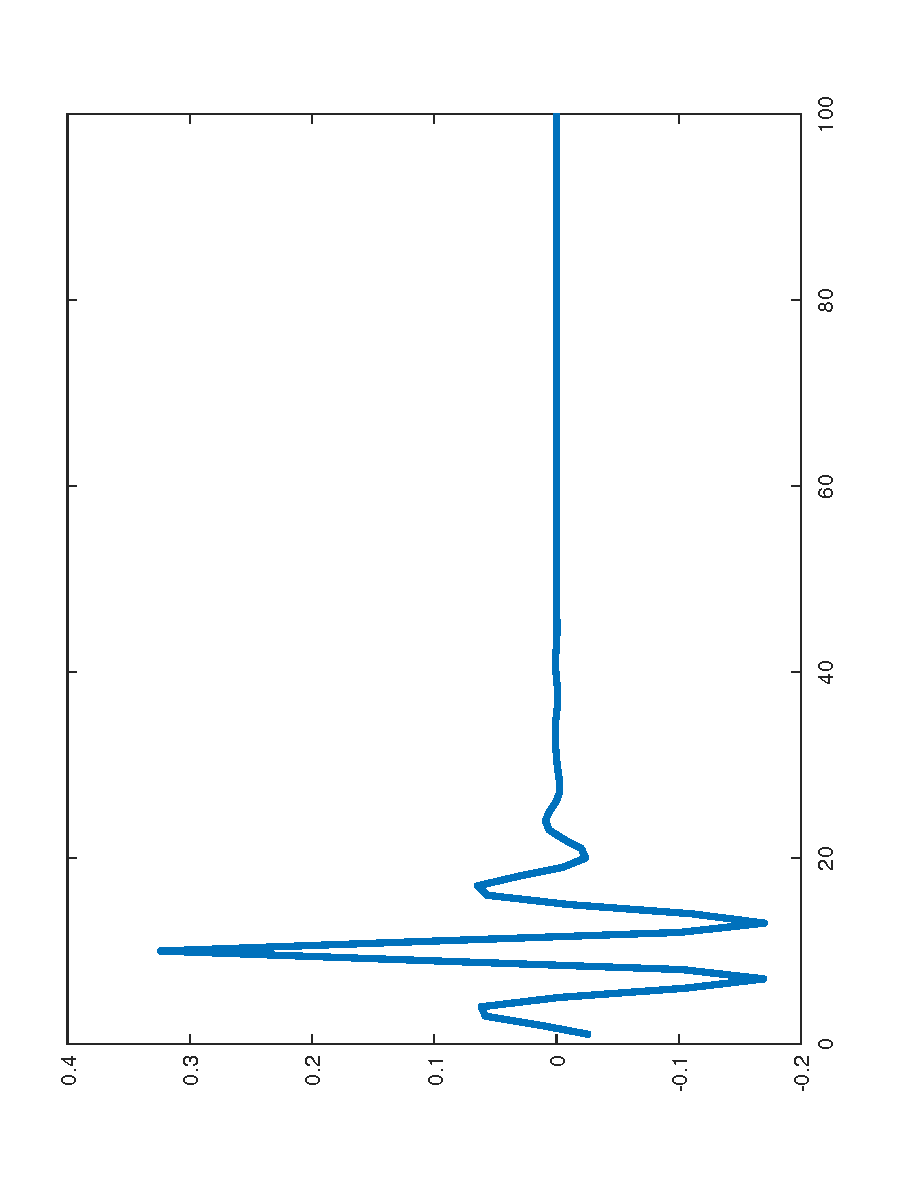
\includegraphics[
        angle=-90,
        origin=c,
        width=\textwidth]{papers/sgwt/images/wavelets-psi-line-4-10.pdf}
        \vspace{-45pt}
        \caption{$\psi_4(v_{10})$-Wavelets eines Streckengraphen mit 100 
        Knoten.}
        \label{fig:sgwt:wavelets:line3}
    \end{minipage}
    ~
    \begin{minipage}[b]{0.49\textwidth}
        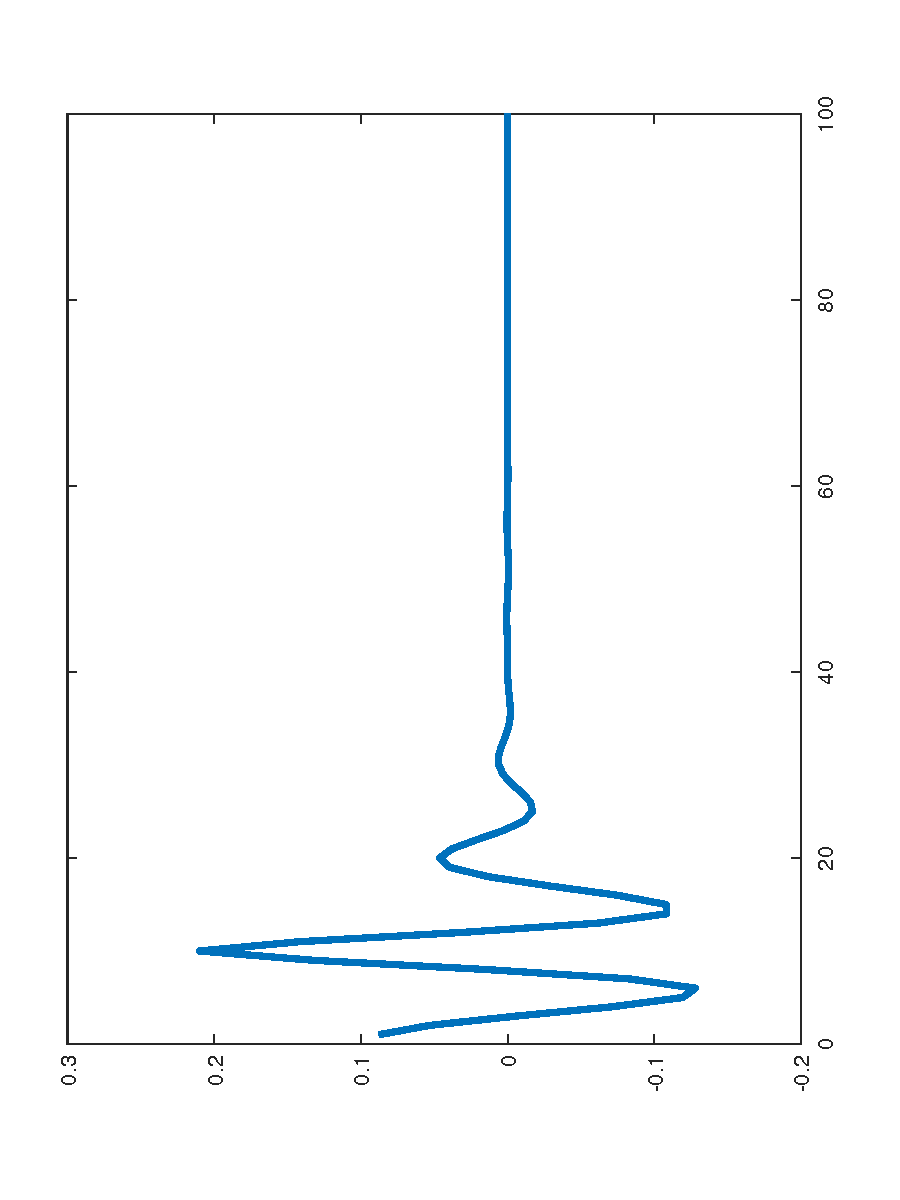
\includegraphics[
        angle=-90,
        origin=c,
        width=\textwidth]{papers/sgwt/images/wavelets-psi-line-5-10.pdf}
        \vspace{-45pt}
        \caption{$\psi_5(v_{10})$-Wavelets eines Streckengraphen mit 100 
        Knoten.}
        \label{fig:sgwt:wavelets:line4}
    \end{minipage}
    ~
    \begin{minipage}[b]{0.49\textwidth}
        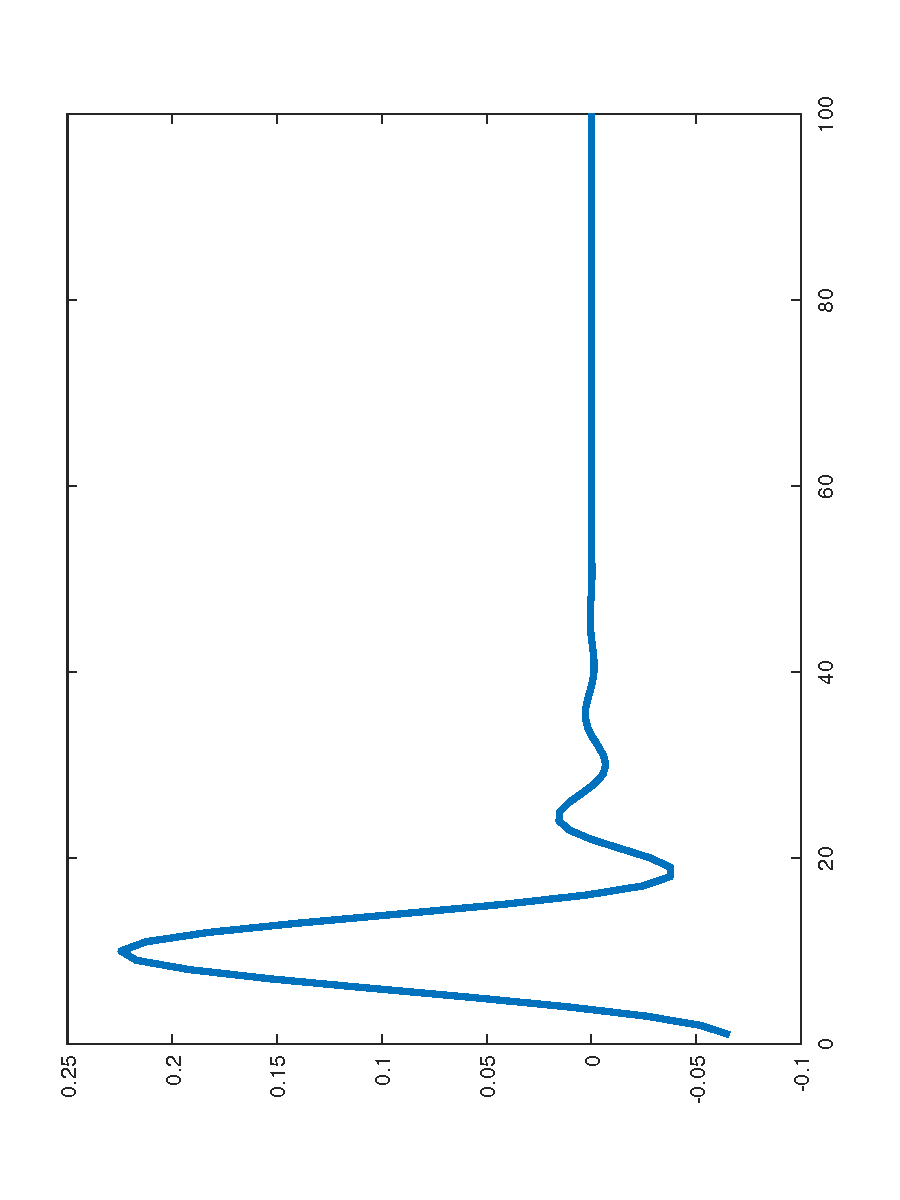
\includegraphics[
        angle=-90,
        origin=c,
        width=\textwidth]{papers/sgwt/images/wavelets-phi-line-10.pdf}
        \vspace{-45pt}
        \caption{$\phi(v_{10})$-Wavelets eines Streckengraphen mit 100 Knoten.}
        \label{fig:sgwt:wavelets:line5}
    \end{minipage}
\end{figure}

Die Wavelets k\"onnen wir dann wieder ein die $N(J+1)\text{x}N$-Matrix $T$ 
packen um dann die Wavelet Koeffizienten wie folgt zu berechnen
\begin{equation}
\hat{f} = T f.
\label{eq:sgwt:hatf}
\end{equation}

\subsection{SGWT Analyse und Synthese}

Um nun eine Funktion $f(v)$ auf einem Graphen $G$ zu analysieren gehen wir 
also wie folgt vor:
\begin{itemize}
    \item[1.] Generierung der \laplaceL{} Matrix aus dem Graphen $G$.
    \item[2.] Berechnung der Eigenwerte $\lambda$ und Eigenvektoren $\chi$.
    \item[3.] Berechnung der $\psi_j$ und $\phi$ Wavelets 
    mit~\cref{eq:sgwt:psi,eq:sgwt:phi}.
    \item[4.] Berechnung der Wavelet Koeffizienten $\hat{f}$ 
    mit~\cref{eq:sgwt:hatf}.
\end{itemize}

F\"ur die Synthese nehmen wir als Eingabe die bei der Analyse berechnet und 
danach m\"oglicherweise bearbeiteten $\hat{f}$. Zus\"atzlich brauchen wir die 
$T$ Matrix, mit deren Inversen wir wieder die Funktion
\begin{equation}
f = T^{-1} \hat{f}
\end{equation}
synthetisieren. Da diese Matrix aber nicht mehr quadratisch ist, kann sie nicht 
mehr so einfach invertiert werden. Wir nehmen uns daher das Pseudoinverse $L = 
(T^*T)^{-1}T^*$ zur Hilfe und erhalten
\begin{equation}
f = L \hat{f} = (T^*T)^{-1}T^* \hat{f}.
\end{equation}


\section{Wavelet-Transformation}

\section{Plancherel-Formel}

\section{Umkehrformel}






